\chapter{Kins}
% Guidelines:
% * At least one page of information should be provided for the kin.
% * Every kin should have at least one illustration to provide visual aid for the player.
% * Every kin must have 7 traits in total.
%   * At least one must be something unique and interesting to the kin (not necessarily useful).
%   * Some kin may have less if they have an extremely good trait (like the ird with a flying speed of 15 meters).
%   * At least one should bring a detriment along with their benefits.
%   * No trait should be purely detrimental.
%   * Some subraces can have detrimental features, but they're countered by good stuff.
% * Kins generally shouldn't lean to one particular playstyle, but this isn't always avoidable.
% * Some description of civilizations related to a certain kin is allowed, but shouldn't be the main focus.

\begin{linenumbers}
\DndDropCapLine{C}{ountless millenia before any of the}
modern kins were born, the ets were born into the land of Yuadrem.
% They were named by the other kins, their creations, due to their impressive size.
They were commonly known as the tall kin, for they usually stood well beyond 3 meters.
Their skin was of a pallid, almost bluish white color, and their eyes were as black as the abyss.
% Most ets didn't have any hair.

The species greatly developed their technology, which was biological in nature.
Free from aging and illness, they developed astonishing physical capabilities despite their apparent frailty.
Each et was indeed capable of shaping their own flesh, causing a great variety of characteristics in the many members of the kin.

Ets were obsessed with their individuality, and it was common for them to change their own appearance, molding their flesh to reflect their personality and philosophy.
Despite their longevity however, it was rare for new ets to be born, and the kin never grew to more than a few thousand members.

\subsubsection{Schools of Thought}
Their longing for longevity led them to study the cosmos, trying to find meaning in the stars.
These studies manifested in the form of the schools of thought, large organizations representing different ways of thinking about the cosmos and oneself.
These schools were their main form of government.%, where individuals were represented by their schools.

Among these organizations, the church of E'ukarilth was of special significance.
More than a thousand years ago, an event known as the first communion took place.
During a pilgrimage to the dead sea, the et E'ukarilth found the deceased embryo of a species yet unknown to its kin, which the tall one dubbed ``the higher kin''.

In an attempt to understand this newfound race, the tall one fused their body with that of the higher one.
The ritual was successful, but it transformed E'ukarilth to an insane, shapeless blob.
Later, the church of E'ukarilth was born to attempt communication with the mad et.

As the gospel of E'ukarilth spread, the kin became convinced that they were utterly insignificant to the cosmos.
The fear caused by this thought elevated their pursuit of individuality.
They believed that the higher kin held a method to become significant, and their schools of thought shifted their studies to focus solely on this strange species.
They believed that with this study they would attain something they called ``the rapture'', described as an ascension to a higher plane of existence.

Their unwavering pursuance eventually led to the schism.
The schism is the most devastating event in Yuadrem's history, causing a 40 year long famine and scarring the land itself for the centuries to come.

\subsubsection{Language}
The tall kin spoke a very sophisticated language, known as jan-theth rlin, simplified as jantherlin.
This language allowed for a very profound expression of one's emotions and inner state, and is still used in poetry to this date.
For when deeper communication is needed, ets could meld their bodies and share thought, but the practice was only used in special rituals or to express especially complex abstract concepts.

As for written word, it was customary for the tall kin to chisel the stone, commonly carving a great variety of images alongside the text.
While this written language originates from jantherlin, each tall one had its own personal version of it.
Other ets could only comprehend one's writing as much as they understood the writer.
This makes the study of jantherlin extremely difficult to modern archaeologists.
% This makes the reading of the jantherlin extremely difficult for the kin that remain in the world, since understanding a particular tall one's scribbles essentially requires understanding their own version of the language.

\begin{figure}[t]
    \centering
    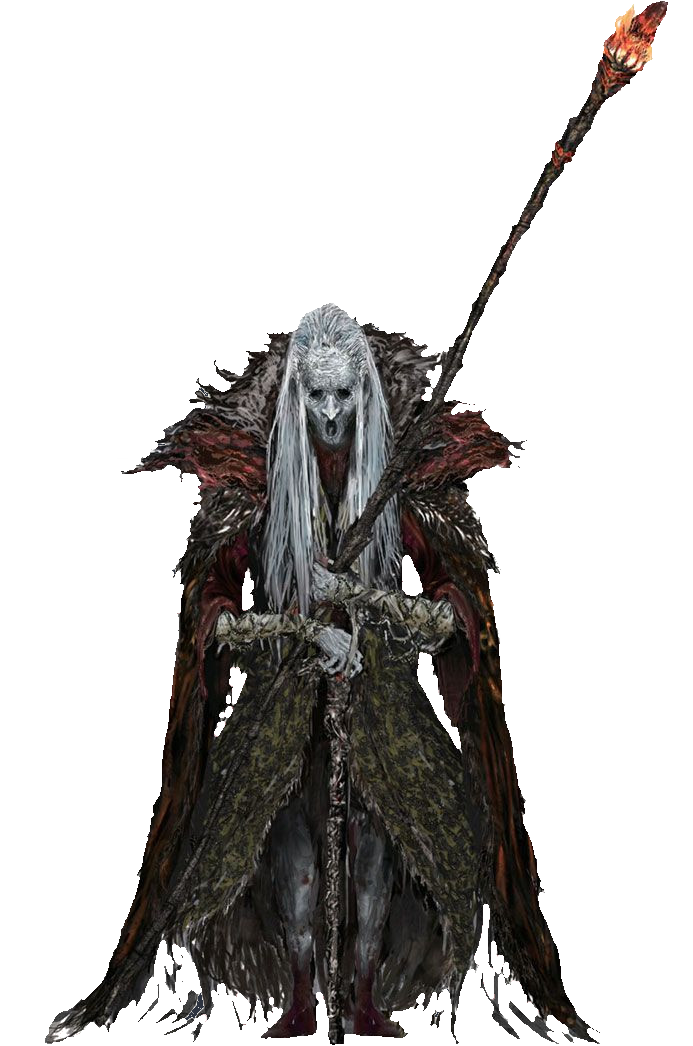
\includegraphics[width=0.45\textwidth]{02kins/img/10et_cleric.png}
\end{figure}

% \subsubsection{Relationships}
% Either by accident or by conscious decision, the tall kin created many of the modern peoples in experiments and studies.
% Most of these held a very high regard for the ets, with some even building entire churches to them.
% However, after it was learned that the they were responsible for the schism, all churches were forcibly shut down, and any adoration is severely punished.
\end{linenumbers}

% TODO: CHECK gats, irds, marsets, and oths and see that any trait that could be considered a technique actually is one, adding it to that list (and padding more text to account for the lost space.
% TODO: I should add an abstract image related to the tide color of each kin as background, which would enhance the relevance of the tides.

\section{Horned Kin}
\begin{linenumbers}
\DndDropCapLine{W}{hen you contract a horned one, be}
\textit{sure to pay them double.
Fulfill all their needs as they seclude into their workshop, and pay no mind to their uncanny silence.
Most of all, be sure to avoid interrupting them.
Just wait.
The prize that will arrive after they're done working is sure to outshine all your other possessions, and hold a special place in your collection for you and your descendants.}

\hspace*{\fill} --- Orr, Vesjen's master smith.

Citadels carved into the highest of cliff faces.
Mines hidden inside the deepest of ravines.
Workshops rumbling with the sound of hard labor until the darkest of hours.
These are the traits that define the gat.

The gat, marheth'llal rlue, or horned kin are the oldest among the sentient races created by the ets.
Molded as diggers and laborers, their passion for work is ingrained into their very blood.
To date they are known as master miners, builders, and artisans.

Being the first of the kins, they are established and well-developed.
Gats are the builders of the Seven Kingdoms of the Coast, the oldest active nations in Yuadrem.

\subsection*{Beard and Horns}
The horned kin was designed in the image of goats, and share their horns, facial features, and digitigrade feet.
They stand in a hunched manner and are generally slender.
Gats are covered by a thick layer of fur ranging in hues from light blonde to absolute black.
Many enjoy growing a beard.

Gats' eyes are of strong colors, usually light blue, yellow, orange, or light brown.
Like goats, their pupils are rectangular and elongated.
The manner in which each gat's beard and horns grow is unique, and most take pride in these features, showing them off whenever possible.

Gats are genderless creatures.
All gats are born with a pair of seeds hidden in a small sack between their legs.
Around the age of 30, a gat reaches physical maturity.
This is signalled by a slight swelling in these seeds, which they can now cut and plant under a thick layer of rich soil.

While underground, the seed will grow by leeching nutrients off the earth.
After a gestation period of around 2 years, the gat will dig their way up from the ground and emerge as a somewhat competent infant.
A gat would-be-parent must always be careful about where to plant their seed, for if a newborn sees the sun or any strong light during their first days, they run the risk of being permanently blinded.

\subsection*{Adaptable and Hardy}
Gat share many traits with the common goat.
They dwell on bleak mountaintops, deep ravines, rocky hills, and open plains.
While adult gats are not sensitive to sunlight, most prefer dark places.
These predilections lead to gat towns and cities being built underground or in harsh cliff faces.

Never satisfied with their homes, the horned kin's hubris leads to their cities to reach depth and size.
Raids against smaller gat city-state are common, and the gats take them as a chance to test their impenetrable defenses, complex traps, and combat-hardened military skills.

\subsection*{Peaceful Demeanor}
The horned kin are peaceful creatures and mostly shun external conflict.
They are very sociable creatures, and all city-states have one large marketplace in their center for merchants and caravans to settle in.
Surrounded by inns and taverns, these markets act as the commerce hubs of the city.

Community lifestyle is very important to gats, and most wouldn't flinch to give their lives for their city-state.
Due to the gats' slow reproductive cycle, their cities are very welcoming to other species.
It's common to find cities and towns where less than half of the total population is gat.
They treat other species as kin, but high political and military ranks are exclusive to gats.

\subsection*{Impulse towards Greatness}
It is rare for a gat to willingly leave their home, and most spend their entire lives in one city-state.
However, some do feel the call to adventure, and most follow it to gather rare crafting materials or to fulfill a task needed by their community.

Gats are meticulous individuals, and this naturally extends to adventurers.
They won't step into the wilderness unprepared, sparing no expense in armor, weapons, utilities, and the training to use all of this.

Gats are naturally family-oriented, and its very rare for one gat to abandon their progeny.
In the rare occasion that a gat does decide to leave their community behind, it is written law to leave one child or seed planted back home.

This tradition serves a double purpose.
First, the child acts as a magnet to their parent.
Second, in the event that the child is orphaned, their mere presence at least maintains a steady population number.
These gats are the ``Children of the Collective'', and it is tradition that they are taken care of by the whole city, thus nurturing a strong sense of community.

\subsection*{Gat Names}
All gat tongues are simple and practical languages, and the horned ones have a tendency towards easy to pronounce names.
A parent gives their child their name once they gain Independence, and its very rare for a gat to change it.
Gats don't use family names, preferring instead to wear their main profession as a surname.

\paragraph{Names} Adrevik, Ani, Anush, Armen, Avag, Gagik, Garen, Gevog, Gohar, Grigor, Hak, Harig, Hovsep, Jirar, Kevon, Khadzak, Marim, Narek, Pagran, Poghos, Ruben, Sivadr, Sona, Vahagn, Vefan.

\paragraph{Surnames} Axgat, Bonecarver, Bowyer, Caretaker, Cook, Dyer, Engraver, Farmer, Fishergat, Glassmaker, Gemcutter, Guard, Mason, Metalsmith, Miner, Speargat, Trader, Trapper, Weaponsmith, Woodworker.

\subsection*{Traits}
Your gat character's hardiness and tendency towards craftsmanship gives them the following set of skills:

\subparagraph{Ability Score Increase} Your Constitution score increases by 2.

\subparagraph{Age} Gats mature slowly, but they live very long lives.
You are sexually mature at around 30 years, and live to around 350 years.

\subparagraph{Alignment} Industrious and strong, gats focus more on getting things done rather than morals or ethics.
They have a tendency towards fairness and justice, and therefore are inclined towards the indigo tide.

\subparagraph{Size} Gats typically range from 1.2 to 1.5 meters.
Your size is medium.
They aren't too slender or stout for their size, weighing on average 50 kg.

\subparagraph{Speed} Your base walking speed is 9 meters.

\subparagraph{Stable Footing} You are not slowed by difficult terrain caused by rocks, gravel, sheer faces, and other such obstacles.

\subparagraph{Force of Will} You can plant yourself in place with all your weight, making you very difficult to move.
As long as your feet are on the ground, you have advantage on any ability checks or saving throws made to move you or force you to fall prone.

\subparagraph{Keratin Horns} You know the Push technique (See page \pageref{tec::push}), using your strong horns to shove your target.
The saving throw the creature must throw is updated to a DC 10 + your proficiency bonus + your Strength modifier.

\subparagraph{Craftsgatship} You learn the first rank of any talent of your choice in the Artisan Talents table (See page \pageref{tal::artisantalents}).
Additionally, crafting times with the artisan's tools related to the talent are halved for you.

% \subparagraph{Gat Resilience} The horned kin possesses an almost otherwordly hardiness.
% You have advantage on saving throws against poison and are resistant against poison damage.

\subparagraph{Strange Mood} Periodically, individual gat are struck with an idea for a masterwork artifact and enter a strange mood.
Only with a great force of will can a gat ignore this pull, and not even the strongest can fully stop the craving.

If you are at least 30 years old, roll a d100 at the beginning of each month.
% You can choose to roll this twice.
On a 100, you are struck by a strange mood.
The materials required for your masterwork item can either be chosen by you or by the DM.
They must be related to the proficiency given by your Craftsgatship trait and at least one of them must be hard to find or very expensive.

At the first day of every month, you must succeed on a Wisdom saving throw of a DC equal to 8 + the number of months since your strange mood started.
On a fail, the need to work on your craft consumes you and you cannot sleep until you either obtain or produce a new material to use in the item, start crafting the item or one of its components, or reach an exhaustion level of 4.

It takes you 2 months of work to craft the artifact, but after you start you can indefinitely pause the production as long as you can properly secure it.
The masterwork item produced has a value of 100,000 GP, but it's very rare to see a gat willingly part with it.
These items are usually declared as family heirlooms, personal keepsake, or an offering to a king, leader, or deity.

Weapons, armor, or similar objects crafted in a strange mood are +2, and are of specially exquisite quality.

\begin{figure}[!b]
    \centering
    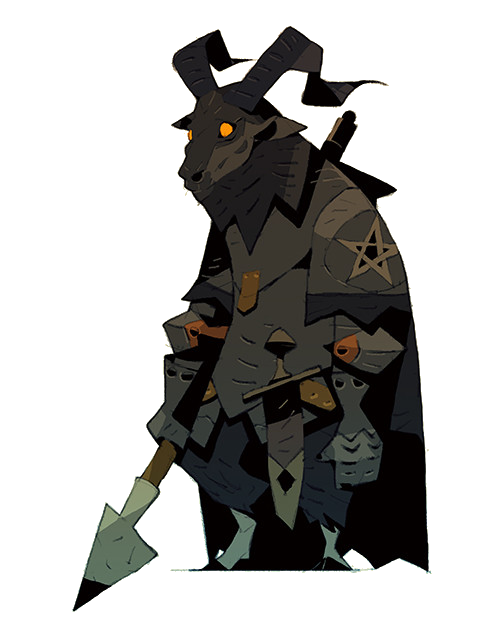
\includegraphics[width=0.47\textwidth]{02kins/img/11gat_knight.png}
\end{figure}

\newpage

\subsubsection{Noves Gat}
Acclimated to the highest mountains and deepest ravines, cliff gats are the most common of the horned kin.
Builders of the immense gat city-states, it's very rare to see a cliff gat not actively pursuing their craft.

\subparagraph{Ability Score Increase} Your time spent in civilization has given you a profound common sense and a general grasp on almost any subject.
Your Intelligence score is increased by 1.

% \subparagraph{Mountain Born} You are acclimated to high altitude, including elevations up to 6,000 km.
% You're also naturally adapted to cold climates, and have a climbing speed of 6 meters.

\subparagraph{Gat Toughness} Your hit point maximum increases by 1, and it increases by 1 every time you gain a level.

\subparagraph{Legendary Craftsgatship} Noves gats are renowned worldwide for their crafts, and even the untrained eye can recognize an item made by one.
You learn the third rank of the talent you chose in the Craftgatship trait.

The value of the item you produce in a strange mood is increased to 250,000 GP.
If you make a weapon, armor, or similar item, it is a +3 item.
Additionally, you must roll your Strange Mood wisdom saving throw twice at the beginning of every month.

\subsubsection{Bughna Gat}
In the year 102 AS, the army of healing invaded Ctereth's dwellings and plundered a great haul of qualar.
These qualar restored the minds of many gats, who became known as the bughna gats.
% While their minds were recovered, the habits they learned as lost ones have never truly been abandoned.

Bughna gats feel constrained in cities, and tend to abandon city-states at a young age, freely exploring the outside world.
% Despite their nature, gats are never truly free of their sense of community.
Bughna gats tend to travel in packs comprised by varied kins and ethnic groups.

\subparagraph{Ability Score Increase} Your balance and ability to walk on the steepest of hills is unmatched, and your Dexterity score is increased by 1.

\subparagraph{Fleet of Foot} Your base walking speed increases by 3 meters.

% \subparagraph{Hardy} You are proficient in the Survival skill.

\subparagraph{See Them Coming} You have advantage on initiative rolls while in plains, grasslands, and any other open natural environment.

\subsubsection{Treb Gat}
While many of the gat lost ones were recovered, most of those who wandered off to the dead sea could never be found due to the toxic mist.
Here they became the Treb Gat, and eventually acquired qualar back via unknown means.

These gats are far removed from their calm origins, having to survive the harsh and hostile environment.
Treb gats have large and muscular bodies, large horns, and dirty, patchy hair.

\subparagraph{Ability Score Increase} Your restlessness knows no bounds.
Your Strength score is increased by 2, and your Intelligence score is reduced by 1.

\subparagraph{Size} Treb gats tend to be much larger than their common brethren, measuring between 160 and 200 cm and weighting between 90 and 120 kg.
Your size is still medium.

\subparagraph{Uncanny Brutality} While in combat, you are absorbed by a primal rage.
You have disadvantage on any attacks made with finesse, martial weapons without the heavy property, and ranged weapons.

\subparagraph{Hammering Horns} You are never unarmed.
Your horns are a melee weapon that deals 1d6 plus your Strength modifier as bludgeoning damage, and you can use a bonus action after a melee attack to attack with them.

\subparagraph{Savage Attacks} When you score a critical hit with a melee weapon attack, you can roll one of the weapon's damage die one additional time and add it to the extra damage of the critical hit.

\subparagraph{Fell Mood} When you are struck by a strange mood, the need to craft an exquisite artifact is replaced by an unrelenting urge to kill.
You have to choose your prey from either a renowned hero, an ancient being, or a forgotten beast.

After the deed is done, you must craft a disquieting artifact from the creature's remains, following the normal rules of a strange mood.
All the other conditions of the trait remain the same, replacing the need to gather materials with the insatiable craving to hunt said creature.

\begin{figure}[!b]
    \centering
    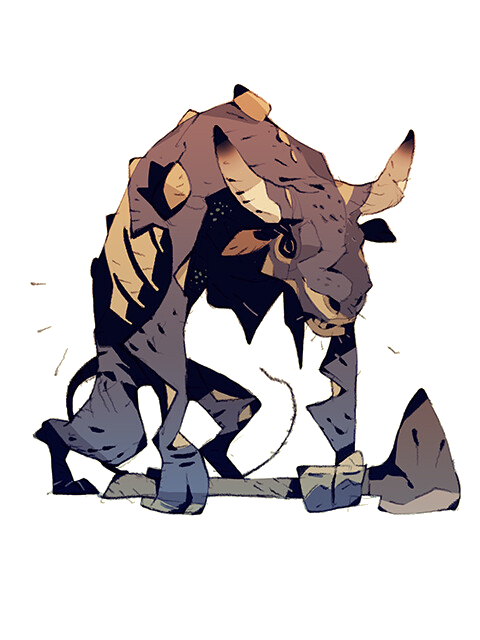
\includegraphics[width=0.48\textwidth]{02kins/img/11gat_treb.png}
\end{figure}
\end{linenumbers}

% !TEX root = ../main.tex
\section{Winged Kin}
\begin{linenumbers}
\DndDropCapLine{Y}{es, sure, you can create a machine to}
\textit{glide.
You can even ride a creature to stay aloft.
But you will never truly fly.
No kin can tame the sky with such grace as the irds.
Trust me, if they weren't so humble as to live among us, constrained to the ground, we'd be building temples to venerate their graciousness.}

\hspace*{\fill} --- Josiah, priest from the church of Rhekesh.

Sequestered in high mountains, deep jungles, and hot deserts, the irds, sisz rlue, or winged kin are known to survive some of the harshest environments all around Yuadrem.

\subsection*{Beak and Feather}
From below, irds look much like large birds.
Only when they descend to roost or walk in the ground does their humanoid appearance reveal itself.
Standing upright, an ird might reach 2 meters tall.
They have long, narrow legs that taper to sharp talons.

Feathers cover their bodies, with their plumage typically reflecting the environment they develop in.
Their heads complete the avian appearance, being that of a parrot, hawk, or vulture.
Irds' arms have very long feathers, which allow them to fly with ease.
The three subraces of the irds are very distinct from each other.
This is due to the fact that they were created by three different ets, all in pursuit of a same goal, yet for different environments.

The winged kin are the only gendered species created by the tall kin.
Some time after reproduction, a female will lay one to three eggs and the couple will refrain from contact with others in their tribe, becoming extremely protective of their children until they reach maturity.

\subsection*{Sky Wardens}
Nowhere are the irds more comfortable than in the sky.
They can spend hours in the air, and some go as long as days, locking their wings in place and letting the thermals hold them aloft.
In battle, they prove dynamic and acrobatic fliers, moving with remarkable speed and grace, diving to lash opponents with weapons or talons before turning and flying away.

Once airborne, an ird leaves the sky with reluctance.
They sometimes forget or ignore vertical distances, and they have nothing but pity for those earthbound kins forced to live and toil constrained to the ground.

The ird are a tribal species, and its rare for a tribe to hold more than a hundred irds at once.
The only exceptions to this rule are the Krudzal and Kaldrathal, both large countries in the northern reaches of Yuadrem.
They are welcoming to traders and visitors in general, but generally don't allow members from other kins to be permanent residents within their territory, and frown upon guests who overstay their welcome.

Once tribes of irds settle in an area, they share a hunting territory that extends across an area up to 150 km on a side, with each tribe hunting in the lands nearest to their colony, ranging farther should game become scarce.
A typical colony consists of one large, open-roofed nest made of woven vines.
The eldest acts as leader with the support of a shaman.

\subsection*{Avian Mannerisms}
The resemblance of ird to birds isn't limited to physical features.
Irds display many of the same mannerisms as ordinary birds.
They are fastidious about their plumage, frequently tending their feathers, cleaning and scratching away any tiny passengers they might have picked up.
When they deign to descend from the sky, they often do so near pools where they can catch fish and bathe themselves.
Even when perched on a high branch or at rest in their mountaintop homes, they appear alert, with eyes moving and bodies ready to take flight.

Many winged kin punctuate their speech with chirps, sounds they use to convey emphasis and to shade meaning.
An ird might become frustrated with people who fail to pick up on the nuances; an ird's threat might be taken as a jest and vice versa.
Confinement terrifies the winged kin.
To be imprisoned by the cold, unyielding earth is a torment few ird can withstand.

\subsection*{Innate Curiosity}
Irds are naturally curious which, summed with their freedom of movement, leads to them being the ideal explorers and adventurers.
They use their large wings to travel to almost any place in the entirety of Yuadrem, and as such they've become a common sight in all its reaches.
Outside of their tribes, irds do enjoy living within other civilizations, and its rare to see a city or large settlement without at least one ird inhabitant.

% Winged kin tribes are accepting of their members leaving for indefinite amounts of time, and this is even encouraged in many communities.
% In fact, the population of a tribe is ever-changing, with the only constants being the eldest members and the shaman.
% This means that neighboring tribes have strong and healthy relations, each coming to aid the ones in need without question.
% Another consequence of their tendency to travel is the versatility of ird artisans, who integrate techniques from all around Yuadrem into their craft.

\subsection*{Ird Names}
Ird names separate into two main categories.
The first resemble their original language, Harualish, and include clicks, trills, and whistles to the point that other kins have a difficult time pronouncing them.
When interacting with other races, they may use nicknames gained from people they meet or shortened forms of their full names.

On the other hands, irds from Krudzal, Kaldrathal, and other civilized lands tend to speak Shanise.
Shanise is a language formed from the interaction of Harualish-speaking irds and Avshenese-speaking gats in the north.

An ird last name is usually simply ``son/daughter of'' followed by one of their parent's name.
Most irds admire their parents, and wear their last names with pride.

\paragraph{Harualish Ird Names} Aera, Aial, Aur, Deekek, Errk, Heehk, Ikki, Kleeck, Oorr, Ouss, Quaf, Quierk, Salleek, Urreek, Zeed.

\paragraph{Male Shanise Ird Names} Aden, Azat, Daneal, Dirkir, Eastean, Goker, Idrahin, Jakod, Jaldor, Jasin, Kuneit, Lutdzu, Nuretin, Nutlar, Rezat, Semir, Shasar, Tajik, Tenel, Tshasin, Unut.

\paragraph{Female Shanise Ird Names} Aise, Asutshan, De\~na, Dilsad, Dorun, Drinja, Eda, Gudlag, Gulden, Hazal, Iris, Katrin, Kisnet, Naina, Nerhe, Sehil, Selna, Sher, Solveag, Tedziye, Zainej.

\subsection*{Traits}
Your ird character has access to different abilities common to all subraces:

\subparagraph{Ability Score Increase} Your Dexterity score increases by 1, and your Wisdom score increases by 1.

\subparagraph{Age} Ird reach maturity by age 14, and don't usually live much longer than 150 years.

\subparagraph{Alignment} Ird have an inclination towards the red tide, which is supported by their adventurous lifestyle.

\subparagraph{Size} Ird are tall, and range from 1.70 to 2 meters.
They have thin bodies and hollow bones, weighing between 40 and 50 kilograms.
Your size is medium.

\subparagraph{Speed} You have a walking speed of 7.5 meters, and a flying speed of 15 meters.
To fly, you can't wear medium or heavy armor, carry heavy weapons, wield a shield or be encumbered.
Since you flap your arms to fly, you cannot use them to attack while flying.
You can use your versatile talons to hold and use simple weapons or spellcasting foci.

\subparagraph{Graceful Landing} Your years of living at great heights have taught you how to fall more gracefully.
You reduce the damage die for fall damage from a d6 to a d4, and you do not fall prone after taking falling damage, unless you are unconscious.

\subparagraph{Keen Senses} You are competent in the Perception skill.

\subsubsection{Qulbaba Ird}
Many irds can be found living in isolated tribes inside the jungles of Yuadrem.
In the east they live in Harual, and in the west in the Jenkashian empire.
Qulbaba ird have a face resembling that of a parrot, and their feathers' coloration depends on their gender.
Males usually have very brightly colored feathers, showing any combination of colors.
Females mostly have dull gray, brown, and dark green feathers, aiding their ability to hide in the jungle.

\subparagraph{Ability Score Increase} Your time gliding between branches and vines has augmented your flying capacity.
Your Dexterity score increases by 1.

\subparagraph{Bright Coloration} As a male, you are competent in the Performance skill.
Additionally, you have advantage on Charisma (Intimidation) checks made against creatures with an Intelligence score of 5 or less.

\subparagraph{Dark Feathers} As a female, you have advantage in Dexterity (Stealth) checks made in dim or dark light or in heavily forested areas.

\subparagraph{Strong Talons} You are competent with unarmed strikes, which deal 1d4 plus your Dexterity modifier as slashing damage on a hit.
Additionally, you have advantage of Strength (Athletics) checks made to climb any surface your talons could reasonably grip.

\subparagraph{Language} You know how to speak, read, and write Qualinese and one additional language of your choice.

\begin{figure}[!b]
    \centering
    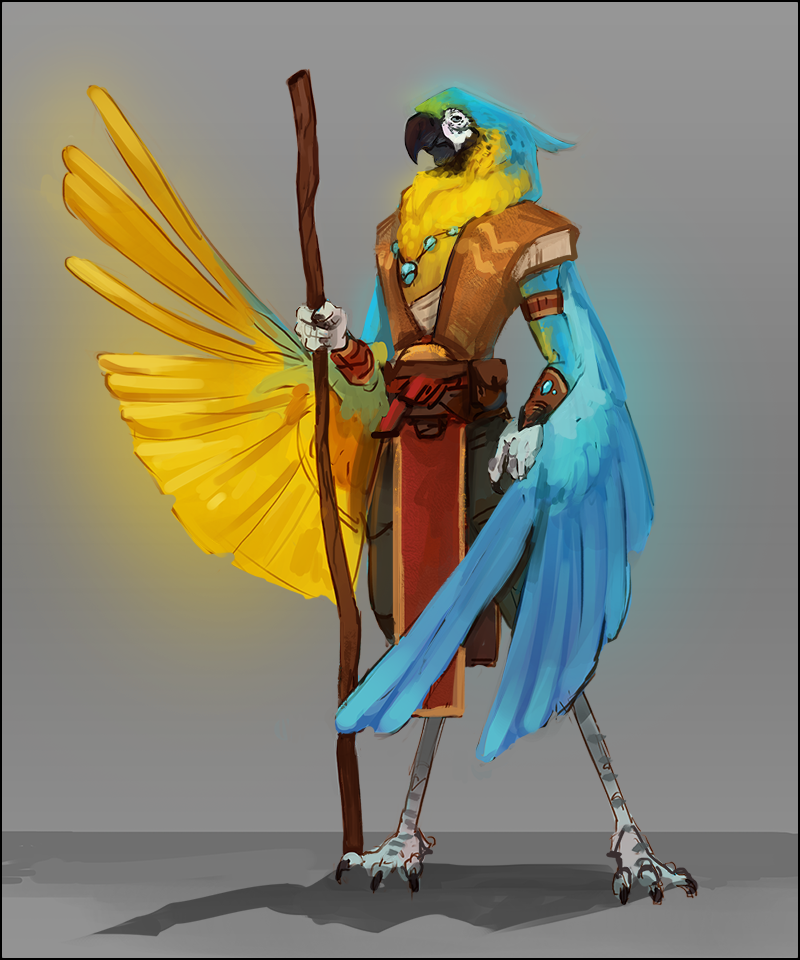
\includegraphics[width=0.48\textwidth]{02kins/img/12ird_qulbaba.png}
\end{figure}

% \newpage

\subsubsection{Thulkraka Ird}
Unlike their brethren, the Thulkraka tribes that settled on the many mountaintops of Yuadrem live their lives mostly constrained to the ground, and are only able to fly when the harsh mountain weather allows it.
They are thus bulkier than the average ird, and commonly are clumsy fliers due to their lack of experience.
Their faces are similar to that of hawks, and their feathers' coloration is bleak and cold, usually sporting white, gray, light blue, and brown colors.

\subparagraph{Ability Score Increase} Isolated from other races, you have been able to take the time to truly appreciate the calmness of the mountains.
Your Wisdom score is increased by 1.

\subparagraph{Bulky Frame} Your flying speed is reduced to 10.5 meters, but you can fly while carrying heavy weapons and/or wearing medium armor.

\subparagraph{Mountain Born} You're acclimated to altitudes up to 6,000 meters.
You're also naturally adapted to cold climates.

\subparagraph{Thulkrakian Descent} You are competent with smith's tools, as is tradition amongst your people.

\subparagraph{Language} You know how to speak, read, and write Shanise and one additional language of your choice.

\begin{figure}[!t]
    \centering
    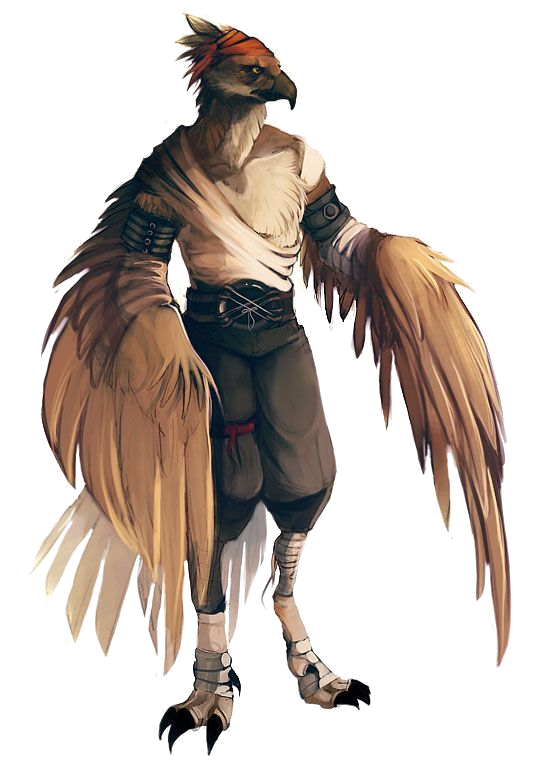
\includegraphics[width=0.47\textwidth]{02kins/img/12ird_thulkraka.png}
\end{figure}

\subsubsection{Dratl Ird}
Irds from the Dratl houses are known as ruthless ruffians, and are pariahs to the other winged kin subspecies.
They are known for constantly harassing the other ird tribes, as well as any who approach their territory.
The are collectively banned from entering any tribe from the other subspecies, and are usually unwelcome in towns and cities due to their bad reputation.

Nowadays, Dratl houses are scattered around the Zoedrem desert, mostly unorganized.
These are the remnants of the once great empire of Hulnar, disbanded in 591 AS.
Despite their lost grandness, they are still feared by the common people, and continue to fiercely protect their hunting grounds.

A Dratl ird's beak resembles that of a vulture, and their feathers are generally black, white, and red.
As a dratl ird grows up, their irises become noticeably white, while the sclera surrounding them turn into a bright red color.

\subparagraph{Ability Score Increase} Your time surviving in the harsh climate of the desert has given you an increased robustness.
Your Constitution score is increased by 1.

\subparagraph{Wing Flap} When you use the disengage action, you can choose to use another action to propel yourself upward a distance equal to half your flying speed.

\subparagraph{Bone Breaker} While flying, you can attempt to attack a creature with an eviscerating attack.
Using two actions, you can swoop down up to your flying speed towards a creature you can see, and make a melee weapon attack roll against it.
If the attack hits, it's a critical hit.
The attack is tiring, and you can use this trait only once per combat encounter.

\subparagraph{Language} You know how to speak, read, and write Zsekian and one additional language of your choice.

\begin{figure}[!b]
    \centering
    \includegraphics[width=0.47\textwidth]{02kins/img/12ird_dratl.png}
\end{figure}
\end{linenumbers}

\newpage

% !TEX root = ../main.tex
\section{Archer Kin}
\begin{linenumbers}
\DndDropCapLine{W}{hile traversing the jungle, be very}
\textit{conscious of your surroundings.
If you stumble upon fiber nests in the trees.
If you hear childlike voices screaming.
Run.
Run as fast as you can.}

\hspace*{\fill} --- Hedwyn's guide to the Chirping Wilds.

The archer kin are a species that resemble large marmosets, barely reaching 90 cm of height.
They share the brown coloration, white ears, and striped tail.
They are small creatures that inhabit the rivers, forests, and jungles of Yuadrem.

They are also known as marsets, or yuathe tle'thal rlue in Jantherlin.
Apart from their size, the other difference from marmosets is their back, which is protected by elongated, pointed quills, used as arrows.

Marsets are an asexual species able to lay eggs at necessity via a ritual after reaching maturity, only limited by the amount of dwellings and social constraints.

\subsection*{Misleading Appearance}
Marsets don't seem terribly intimidating at first glance.
They however have an unusual defense mechanism for driving away threats, which includes any unfortunate creature that disturbs their large arboreal colonies.

Each marset grows specialized quills from their back, with a smooth tip and a base with four flanges, like the fletching of an arrow.
In additional to making the marsets quite painful to grab, these quills are used as projectiles.

The little creatures construct their own bows, stripping bark from bendy twigs with their teeth to create the limbs, and harvesting spiderweb for the string.
The strands are rubbed together with sand, which is done to thicken the bowstring and reduce stickiness in the middle, creating a sophisticated weapon to launch quills at unlucky foes.

For shorter range, marsets also use hollow reeds to blow their quills as darts.
It's common for the smarter marsets to apply manure or poison to their arrows and darts, improving their deadliness.

\begin{figure}[!b]
    \centering
    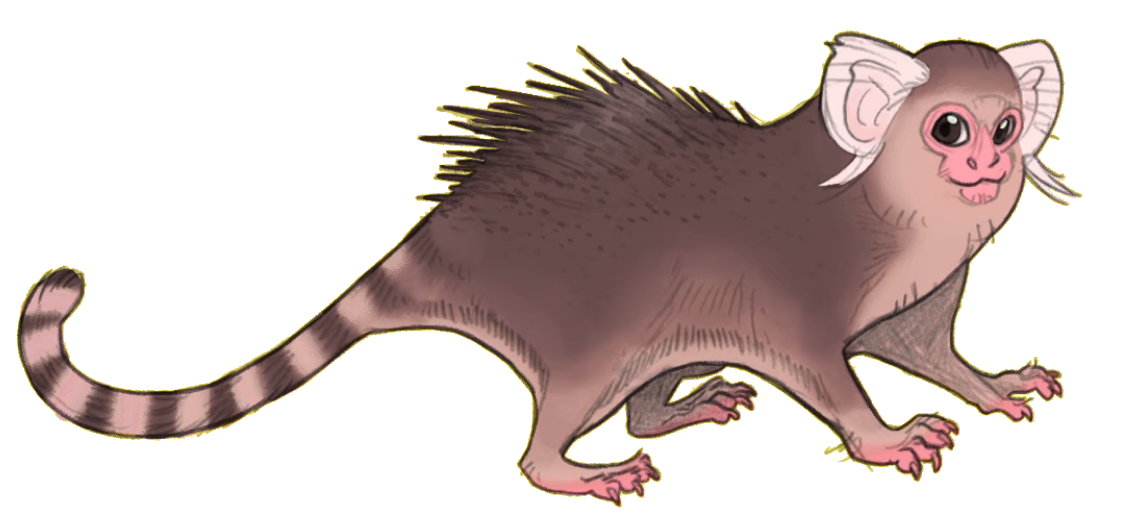
\includegraphics[width=0.48\textwidth]{02kins/img/13marset_brown.png}
\end{figure}

\subsection*{Arboreal Colonies}
The colonies that the marsets protect are just as complex as their weapons.
The structures are created from weaving grass and plant fibres around tree branches to create interconnected chambers.

A single colony can have up to 100 rooms and even more individuals living in it.
Rooms are assigned a specific function, and are passed down through related members of the colony.

Nursery rooms are where marsets lay their eggs, which they hatch into fluffy yellow infants.
Bedrooms are where the adults sleep.
Storage rooms are where food and various items are stockpiled.

In farming rooms they deposit a mixture of tough chewed leaves and bark, which then grows mushrooms.
The little marsets use these rooms to turn otherwise inedible foraged material into something tender and tasty.

While most marsets can be found in these colonies, some choose to live in cities and towns from other civilizations.
Here, they usually build interconnected rooms in trees, creating microcosms of the larger colonies.
Despite their fierceness in their natural environment, marsets are generally regarded as friendly creatures when encountered in urban settings.

\begin{figure}[!t]
    \centering
    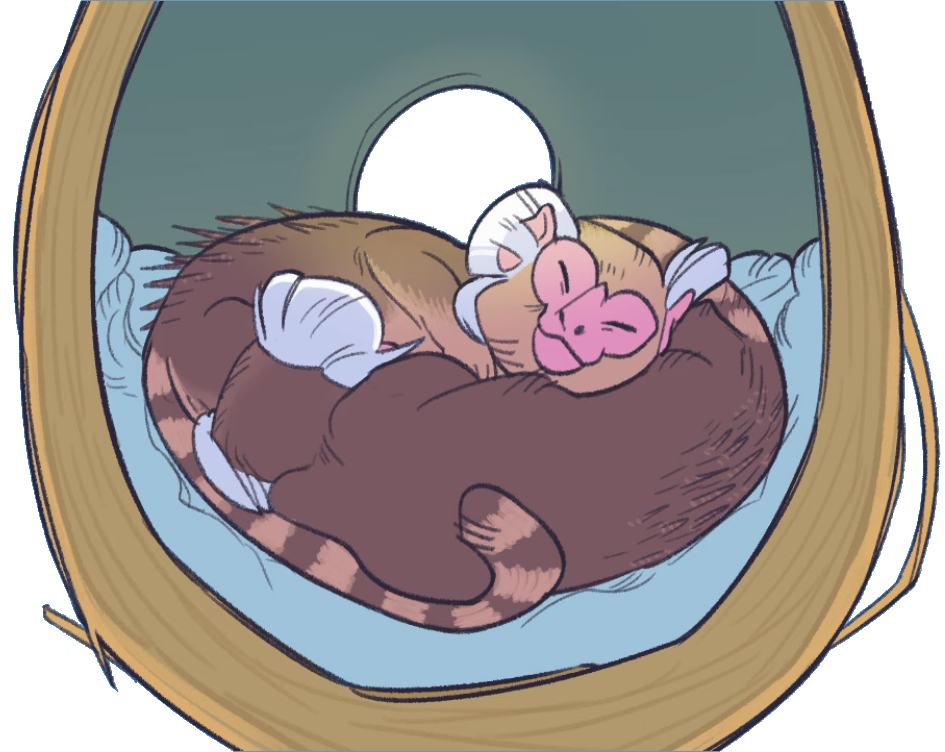
\includegraphics[width=0.48\textwidth]{02kins/img/13marset_room.png}
\end{figure}

\subsection*{Repetitive Language}
Marsets hatch from their eggs already able to speak a strange repetitive language, which is entirely regular and does not evolve.
This language --- known as Babazano --- can be spoken in one of two ways: soundlessly, with the communication happening through lip reading, or screamed as loud as possible, with no middle ground.
Despite this, a marset can learn other languages and not constantly scream at the top of their lungs, but they do tend to be loud speakers.

Babazano has only ten consonants.
All verbs use a single consonant as their root, so there's only ten verbs.
By repeating syllables they create new meanings, which makes their language very difficult to understand by the other kins, but for these little creatures it's no issue at all.
They hear or lip-read a word and instinctively know which one it is.

\subsection*{Exploring Opportunities}
Marsets don't usually set out on the adventurer's path for leisure, but rather out of necessity.
They will only leave their colonies to defend their communities or support their friends.
Only very few will set out to explore the wide world.
% For them, adventuring is less a career than an opportunity and more of a necessity.

\begin{figure}[!t]
    \centering
    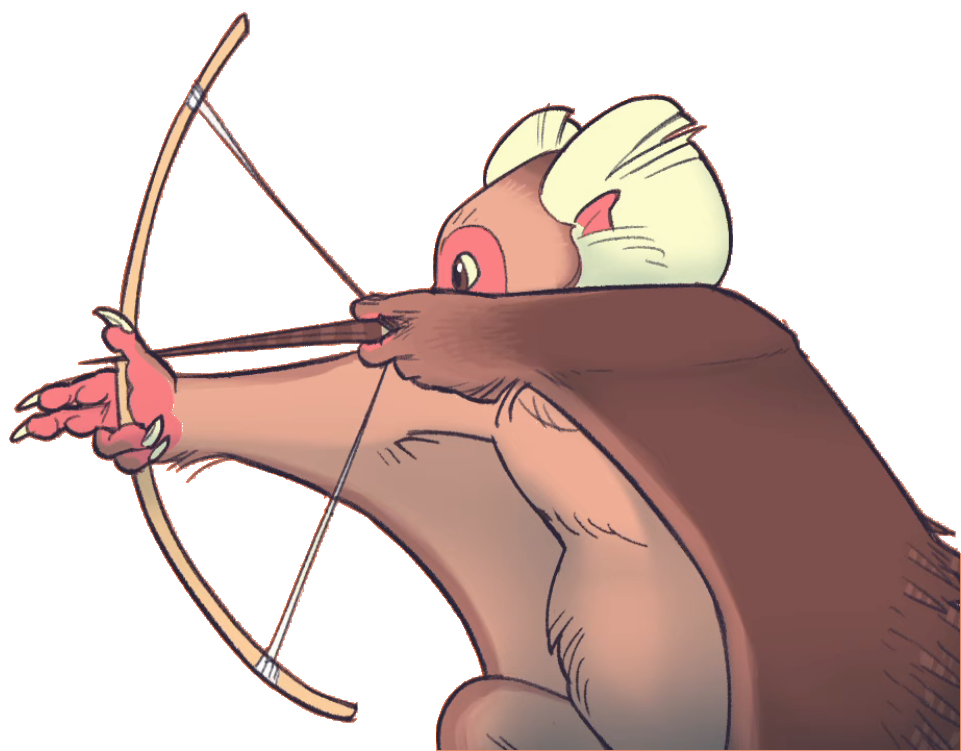
\includegraphics[width=0.48\textwidth]{02kins/img/13marset_bow.png}
\end{figure}

\subsection*{Marset Names}
Marsets assign names to each other based on distinctive features and accomplishment.
An individual marset will wear many names during their childhood, and when they settle on one is when they reach adulthood.
Due to the peculiarity of Babazano, it is a common for the other kins to call them by simple monikers, practice that the marsets despise.
% Most marsets don't particularly like this, and are very reluctant to accept a nickname given to them.

\paragraph{Names} Do Anana, Do Baba, Do Badada, Do Ebebebebe, Do Ezeze, Do Nono, Do Odododo, Do Uvu, Do Veve, Do Vovovo.

\subsection*{Traits}
Your marset character has a range of abilities based on its nature and community lifestyle.

\subparagraph{Ability Score Increase} Your Charisma score is increased by 2, and your Dexterity score is increased by 1.

\subparagraph{Age} Marsets has a short lifespan, reaching maturity by age 4 and not living much more than 50 years.

\subparagraph{Alignment} Marsets have a tendency towards helping others, specially in their communities, and are inclined towards the gold tide.

\subparagraph{Size} Marsets range from 75 to 90 cm.
They usually have a slender and agile frame, weighing around 20 kg.
Your size is small.

\subparagraph{Speed} Your base walking speed is 9 meters, and you have a climbing speed of 9 meters.

\subparagraph{Glider} You have loose flaps of furry skin between your arms and legs, which allow you to glide short distances at a speed of 9 meters per turn, as long as you are not wearing heavy armor.
You fall at a rate of 6 meters per turn while gliding, and suffer no falling damage on landing.

\subparagraph{Sneaky Nature} You have advantage on stealth checks in heavily forested areas.

\subparagraph{Natural Weapons} You are proficient with shortbows and blowguns, and can use your own quills as arrows or cut them to be used as darts.
Every day you can gather up to 10 quills from your back to be used in this fashion.

\subparagraph{Community lifestyle} Despite their loudness, marsets can be very compelling talkers.
You are competent in the Persuasion skill.

\subparagraph{Languages} You can speak Babazano from birth, and can lip-read the language.
You are also able to read and write Leafrunes, a special writing system designed to communicate simple messages to others of your kin.
Additionally, you know how to speak a language of your choice, but you don't know how to read or write it.

\begin{figure}[!b]
    \centering
    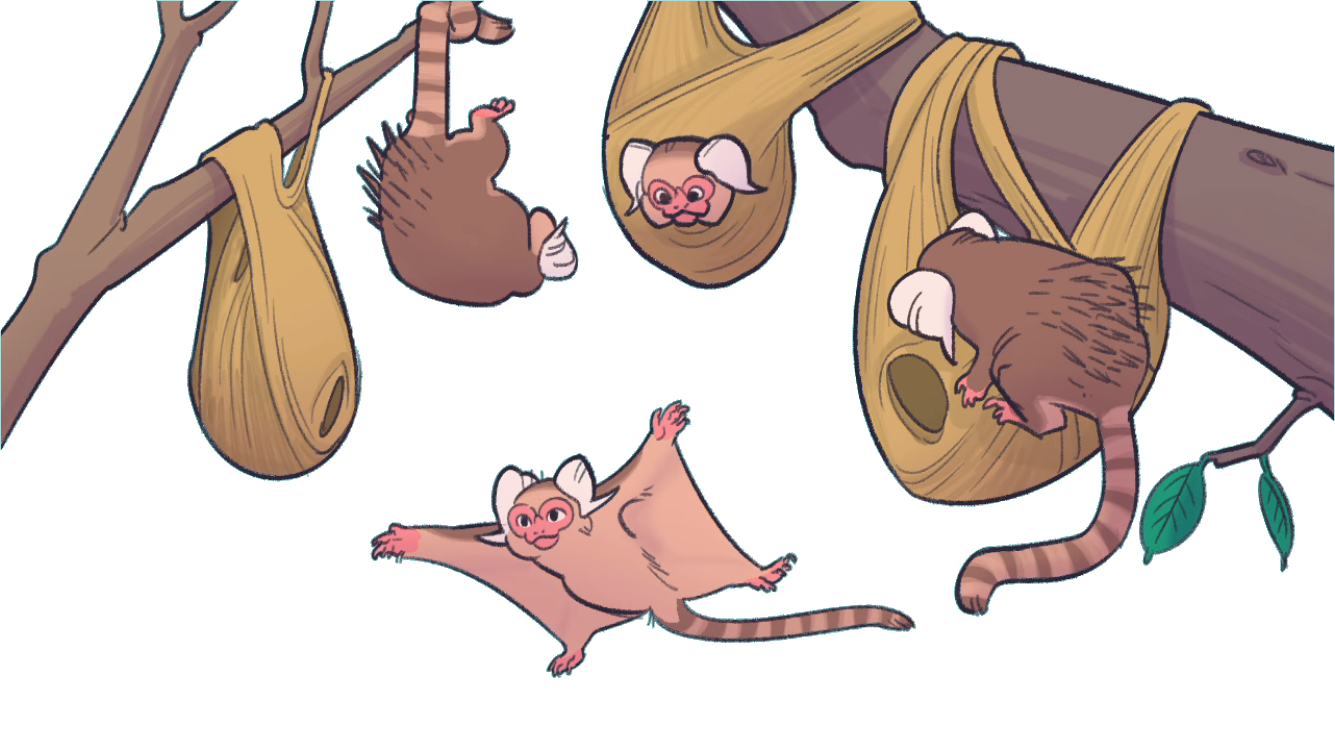
\includegraphics[width=0.48\textwidth]{02kins/img/13marset_colony.png}
\end{figure}
\end{linenumbers}

\newpage

% !TEX root = ../main.tex
\section{Dust Kin}
\begin{linenumbers}
\DndDropCapLine{T}{he light beckons, and you follow.}
\textit{As the light lead you once, now you are guided by enlightenment.
With each hidden truth you uncover, you learn more of what the world is, and how to secure your place in it.
Secrets are your power and your currency.
Seek them out, and guard them well.}

\hspace*{\fill} --- Ancient Moonborn saying.

Moody and perplexing.
Isolated and elegant.
Tough and passionate.
The ways in which one might describe the dust kin are many.
The dust kin, oths, or szua-tlekeloo rlue are a quiet species with a tendency towards nature and knowledge.
They're a solitary yet intimate creature with a penchant for nature and ritual.

\subsection*{Enigmatic and Uncanny}
While oths can be see as much as gats or irds around civilized lands, they are far more mysterious and reclusive than the two.
Often silent, oths have a reputation for being cryptic and thoughtful.
They tend to follow their intuition on a whim.

Oths usually travel with a large scroll in their backs made from their own fabric, which they protect with impermeable and resilient guards.
This scroll is a compendium of knowledge passed down through generations, and they add to it in key moments in their life.

The dust kin have large, heavy forewings that hang around their humanoid bodies like cloaks, which hide a shorter and more delicate set of hindwings behind them.
They have two sets of arms, one above the other.
The upper pair is strong and long, while the lower one is weak, and mostly left for secondary tasks.
Their feet have three fingers and their arms have four, with one being an opposable thumb.
They have an insectoid face with antennae and compound eyes.
Their body is covered in a short, fluffy hair which is usually of a very pale brown color.

\subsection*{Long Tempers}
Through generational learning, oths are wise and prudent creatures from a very early age.
Many chase intellectual or mindful pursuits, becoming librarians and philosophers.
They pontificate on the nature of life and knowledge.
Most think that the oth are naturally intelligent, and take their opinions with very high regard.

While most dedicate to cultivating their cognition, some decide to live their lives in adventure.
They nurture their minds with experience, acquiring knowledge via facing the challenges of the world.

A common thread throughout the race is that they are slow to anger.
Regardless of culture, it is instilled in them as early as the larval stage.
Life is too short to be spent in anger or frustration.

\subsection*{Cycle of Resurrection}
An oth knows when their natural death approaches, and faces it peacefully.
When they are near their death, they say their goodbyes and withdraws from civilized society.
The oth then pilgrimages towards a cavern or secret place they designated during their lifetime.

On arrival, the oth blocks all but one entrance to this sacred place, and lays ten to twenty eggs in a bed of silk during fall.
They then spend their time gathering foodstuffs and lining the walls, floor, and roof with silk, providing a safe environment for their descendants to develop in.
The oth also uses this time to finish writing their compendium of knowledge in their scroll, developing it until its ready to be passed on to their strongest descendant.

At the last week before the break of summer, the oth closes the last entrance to its sacred place, engulfing it in total darkness.
And they wait.

At some point during summer, the eggs hatch for their parent to greet and nourish their newborn larvae.
They dying oth hands qualars to their progeny, teaching them their language and the way of the world.
Along with this they pass on the tenets of their culture.
The parent eats no more than a grain of rice per day, and refrains almost completely from liquids.

Six months after hatching, the younglings go through the process of pupation, remaining as pupa for a year.
The parent uses this time to drink an embalming fluid, and mummifies themselves in silk.
They slowly lose their sentience, peacefully drifting into non-existence.

After hatching, the oths pay tribute to their now dead parent, and re-seal their cradle.
The first place they see becomes their parent's final resting place.
The oths then travel together, forming a small familiar tribe which lasts until they reach maturity.
While the members of the family may part ways, the bond they share is never truly broken.

\subsection*{Educated by Experience}
Due to the way the oths spend their youths, they are generally very wise from a very young age, blessed with the knowledge of the previous generations.
However, it's in an oth's nature to cultivate this wisdom with a contemporary and personal viewpoint of the world.
It's rare to see an oth not spending much of their youth travelling for knowledge and wisdom.
% The dust kin is also very concerned about the preservation of nature, and are experts at recording its sights and dwellers in great detail.

\subsection*{Oth Names}
In oth culture, the parent is assigned the task of naming each of their children in their larval stage.
These names will often change at the whim of the parent, not becoming official until pupation.
Their names are often difficult to pronounce by the other kins, and most don't mind being called by a nickname for simplicity.
The dust kin doesn't use family names, recognizing their relatives by sight alone.

\paragraph{Names} Adz'kt, Andle, Axa, Bixi, Chch, Chith, Daph, Fen'kt, Fl'ka, Fra, G'zigg, Gl'rik, Hadae, Iitus, J'llkx, Kl'il, Lenna, L'kpha, Mlf, N'kakt, Riz, Scelkt, Sud'kx, Thm, Timpth, Zkx.

\begin{table*}[b]%
    \begin{DndTable}[width=\linewidth, header=Oth Silk Armor]{lXXXX}
        \textbf{Armor} & \textbf{AC} & \textbf{DC} & \textbf{Time taken} & \textbf{Cost} \\
        Silk Armor                & 11 + Dex mod     & 10 & 1 week   &    -    \\
        Reinforced Silk Armor     & 12 + Dex mod     & 15 & 2 weeks  &   10 GP \\
        Exquisite Silk Armor (+1) & 12 + Dex mod + 1 & 20 & 1 month  &  100 GP \\
        Excellent Silk Armor (+2) & 12 + Dex mod + 2 & 20 & 6 months & 1000 GP
    \end{DndTable}
\end{table*}

\subsection*{Traits}
Your oth character has the following set of skills, based on its customs and ancestry.

\subparagraph{Ability Score Increase} Your Intelligence score increases by 2.

\subparagraph{Age} An oth will go through three stages of growth: eggs, larvae, and pupa.
This development takes in total about two years.
In terms of maturity, they emerge from their pupa as adults, but reach full size at about ten years of age.
Oths live to be around 80 years old.

\subparagraph{Alignment} Oth tend to stray from extremes, most often remaining neutral in conflicts as long as there is no direct danger to themselves or those close to them.
The oths passion for wisdom leads them to the blue tide.

\subparagraph{Size} Oth typically range from between 135 to just under 180 cm.
Your size if Medium.
You are impressively lightweight for your size, weighing around 45 kg.

\subparagraph{Speed} Your base walking speed it 9 meters.

\subparagraph{Clumsy Flight} Once per short rest, you can fly with a speed of 7.5 meters for a number of rounds equal to your Constitution modifier plus 2, with a minimum of 2 rounds.
You cannot use this feature while you wear heavy armor or carry heavy weapons.

\subparagraph{Darkvision} Due to your nocturnal heritage you have a good sense of vision in the dark.
You can see in dim light within 18 meters of you as if it were bright light, and in darkness as if it were dim light.
You can't discern color in darkness, only shades of gray.

\begin{figure}[!t]
    \centering
    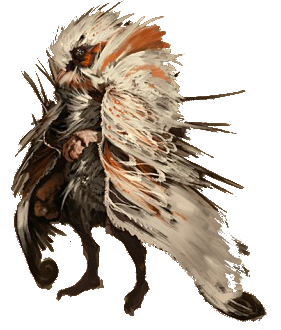
\includegraphics[width=0.48\textwidth]{02kins/img/14oth_white.png}
\end{figure}

\subparagraph{Four-armed} You have a pair of weaker secondary arms that can be used to hold small objects or perform simple tasks.
You cannot use these arms to wield weapons or shields and Strength checks using them are made with disadvantage.
Due to your unique form, armor may need to be specially made, leading to additional costs.

% \subparagraph{Long-lasting Tradition} You are proficient in the Religion skill.

\subparagraph{Silk Spinning} You have the Weaver talent at rank 1 (page \pageref{tal::weaver}).
Dust kin's silk is known for its beauty and strength, and your character can craft cloths and various items with it.
Given enough time, you can craft thread, ropes, bags, clothing, and nets using it.
You can also attempt to weave light armor using this silk, for which you use a set of Weaver's tools.
To successfully craft the armor you need to succeed on an ability check using your Weaver's Tools.
There is a cost associated to the process, relating to the additional materials needed to complete the armor.
The cost is spent at the beginning of the craft, and the DC must be succeeded at the midpoint of the weaving process.

Excellent silk armor requires expertise with Weaver's Tools.

\subparagraph{Silent Speech} You can communicate with other oths and some insectoids using the Silent Speech.
This language can only communicate simple ideas, and it does so via a combination of pheromones and thrumming sounds made with antennae.

\subsubsection{Moonborn}
The moonborn are the most common of the oth.
They prefer shady areas, and tend to live their lives in such places.
They have been properly schooled under the light of the moon as oth tradition dictates, and many can be found in darkened libraries during daytime.

As their name suggests, moonborn have a special affinity for the moon, and can even feed off its light.
They travel at night and hide during the day, and most carry a specially designed tent that blocks all incoming sunlight.

\subparagraph{Ability Score Increase} Your Wisdom score is increased by 1.

\subparagraph{Light Sensitivity} You are vulnerable against radiant damage.
You have disadvantage on attack rolls and Wisdom (Perception) checks that rely on sight when you, the target of your attack, or what you are trying to perceive is under direct sunlight.

\subparagraph{Sensitive Antennae} Using your specialized antennae, you have advantage on perception checks that rely on smell.

\subparagraph{Lunar Studies} You know the first rank of the Pious talent (Page \pageref{tal::pious}).

\subparagraph{Photosynthesis} While you need water like any other creature, you don't need to eat to gain sustenance.
You can choose to instead collect light with your wings via photosynthesis.
Each day, you must spend two hours with your hindwings exposed to sunlight, or four hours to moonlight to be properly well fed.

\subparagraph{Moon Magic} You know the Light cantrip (page \pageref{spell::light}).
When you gain your third hit die, you learn the Faerie Fire spell (page \pageref{spell::faeriefire}), which you can cast once per day.
When you get your fifth hit die, you learn the Glitterdust spell (page \pageref{spell::glitterdust}), which you can cast once per day.

Intelligence is your spellcasting modifier for these spells.

\subsubsection{Chu'ash Kin}
The chu'ash oths are a subculture that differentiate from the rest by their curious and reckless nature.
Weaker than their siblings, they are born a summer too late, and never get to meet their parent.
They are instead cared for by their older siblings, and are the younger members of their familiar tribes.

To most, a chu'ash oth seems perpetually disorganized and distracted, which leads to the belief that they have a lower intelligence to the other of their kin.
In truth, the chu'ash have a unique perception of the world.
They are able to interpret information in a unique way, allowing them to see possibilities other cannot.
Born with an untamed intelligence, the chu'ash oth has an affinity to find the hidden patterns of the world.

\subparagraph{Ability Score Increase} Your Charisma score is increased by 1.

\subparagraph{Touched} You know the Dancing Lights cantrip (page \pageref{spell::dancinglights}).
When you gain your third hit die, you learn the Color Spray spell (page \pageref{spell::colorspray}), which you can cast once per day.
When you get your fifth hit die, you learn the Blur spell (page \pageref{spell::blur}), which you can cast once per day.

Charisma is your spellcasting modifier for these spells.

\subparagraph{Fated} Whether luck of a guiding presence, you always seem to find your way.
Once per day you can choose to reroll any attack, skill check, or saving throw.
You can decide to do this after the roll, but before the outcome of the roll has been determined.

\subsubsection{Sunstruck Oth} % TODO: NEEDS A SLIGHT REWORK
While most oths follow the circle of resurrection to the letter, there are a few who choose to ignore it.
They lay their eggs under direct sunlight, and their larvae quickly lose their fragile hindwings.
Unrepairable, their wings stay atrophied and shriveled thorough their lives.

These oths are known as the sunstruck, and they've earn a reputation of unpaired hardiness and resilience.
The clans of Shief and Zmiva cherish this attribute, and consciously molt in lit areas to engender it.

\subparagraph{Ability Score Increase} Due to your hardiness, your Constitution score is increased by 1.

\subparagraph{Sunstruck Birth} You lose your \textbf{Clumsy Flight} and \textbf{Darkvision} traits.

\subparagraph{Sunstruck Resilience} You know the first rank of the Survivor talent (page \pageref{tal::survivor}).

\subparagraph{Vertical Takeoff} As an action, you can use your powerful frame and knowledge of thermals to propel yourself upward a distance equal to double your movement speed.
This technique is used by the Shief scouts to survey the desert around them in search of food or predators.

\subparagraph{Glide} While useless for flight, your shriveled wings allow you to slow your fall and glide short distances.
When falling, you can use your bonus action or reaction to lift your wings using your second pair of arms to slow your descent.
You continue to fall gently at a speed of 9 meters per round, taking no fall damage when you land.
If you would fall at least 9 meters in this way, you can glide up to your movement speed in any direction you choose except upwards.
You cannot glide if you are wearing heavy armor, or are encumbered.
\end{linenumbers}

% !TEX root = ../main.tex
\section{Moss Kin}\label{src::naenk}
\begin{linenumbers}
\DndDropCapLine{W}{e thought they were mindless}
\textit{savages, but they know what they're doing.
They ain't hiding from us, they're preparing an attack.
They're studying our movement, figuring out our tactics.
They're hunting us.}

\hspace*{\fill} --- Grigor, Drejeck expedition leader.

The moss kin, or naenks, are moss creatures that hunt in the dark, warm, and wet jungles of Drejeck.
They hunt for sustenance and to gather fresh corpses.

\subsection*{Short and tangled}
The naenks are mostly known for their strange reproduction.
They spawn from the corpses of hunted humanoids exposed to the nanust spores of the great tree Tekatsae.
The spores grow into moss, merging with the corpse's muscle tissue and flesh.
After a period of about two months, the corpse rises again, this time in the shape of a naenk.

The moss kin are a thin race.
Their height varies considerably, but they usually are slightly smaller than their birth corpse.
Their bodies mock a humanoid shape, made up by a mix of bone, flesh, vine, and moss.
They protect their fragile interior with thick layers of flora.

Naenks typically have a healthy green coloration, but their skin can be of any mix of colors between moldy blue, dark orange, gray, and even white.
Their eyes are of a white or yellow color, where a thick fluid hides their pupils from the eyes of others.

Naenks naturally grow leaves and mossy tendrils at the top of their heads that resemble hair, which can be of a black, brown, or yellow color.
They typically arrange this mock-up of hair in a simple topknot.

% Due to the duality of their bodies, naenks follow a very particular diet.
% They needs to regularly consume meat in order to maintain the corpse inside them.
% They also feed off nutrients from the soil to feed the vines and plants that surround this corpse.

\subsection*{Tribal Communities}
% A naenk also assists their communication with rhythmic tapping on their body and using a complex system of gestures.
% Apart from these, they can also speak telepathically when close to tsaneks or sovereigns, aiding their communication.

Naenks are organized in tribal units called bands.
Each band is lead by the strongest naenk, the chief, who commands alongside a tsanek shaman.
Naenk chiefs bear special spores that can be used to infect beasts in a manner similar to the Tekatsae tree.
They spawn a bestial moss creature known as nuen with this spores, who acts as a pet or mount to the chief.
When a naenk travels alone, it is usual for them to also grow these spores as well.

Naenks build and craft very little.
Their gear is simply what they loot, and they build simple structures by imitation.

Due to their odd appearance and homicidal reproduction, naenks are seen as something to fear.
They however are very bold, yet fear the strangest things due to superstition.

Strangely, if they remain inside Drejeck, a naenk will not need to carry a qualar to remain sentient.
This ability only works inside of the jungle however, and they quickly lose their sentience if they leave their home without a qualar.

\subsection*{History and Legends}
To become part of a band, an infant naenk needs to go through a unique ritual.
A tsanek shaman removes their thyroid cartilage, who then punctures an odd pattern of holes into it.
After fitting small wooden tubes into these holes, the cartilage is put back into its original place.
After healing, the naenk's voice becomes accompanied by an eerie whistling noise, which is used for communication and intimidation.

Later, the naenk joins a group of other would-be-warriors.
They leave the safety of the tribe to travel to the northern lakes of Drejeck.
In there they must hunt a whowie, a huge frog-like beast that preys on the moss kin.

While they are fierce beasts, whowies are very afraid of the naenks' whistling, aiding the latter in combat.
If the group succeeds, the bravest of the group will cut the whowie's tongue.
Upon returning to the village, the group becomes a new band, and the owner of the tongue becomes the band's chief.

\subsection*{Call to Adventure}
A naenk rarely leaves the Drejeck jungle in which they are born.
However, many reasons can spark the need for a naenk or an entire band to abandon their home.
A band may leave engaging on a quest, as commanded by Tekatsae itself, or in shame after failing in one.
The most common bands abandoning the tribe are those that failed on their initiation rite, culled by the vicious whowie.

While in groups they may be savage, individual naenks are not completely insensitive people.
It is not too rare for a naenk to abandon their tribe in search for a different life.
Discontent with their chief, tiredness from their class system, or mere curiosity of the outside world count among the most common reasons for a naenk to travel by themselves.

% Only known among the naenk and the tsanek is the fact that a huge qualar lies inside the tree itself, which imbues the colossal plant with sentience.
% How this object ended up inside the tree is unknown, but it is thought among them that the tall one cter-rheth is looking to recover it.
% Due to the fact that the kin can't reproduce by themselves, they protect the tree with their lives and, under normal circumstances, won't allow anyone to even approach it.

There is an old legend of a courageous band that will one day sneak into Ctereth's lair and steal a huge bounty of qualars.
These will be used to grow a second tree, brother to Tekatsae, improving the kin's survival by a large margin.
Many groups have tried to become this band of legend, but none has returned thus far.

\begin{figure}[!b]
    \centering
    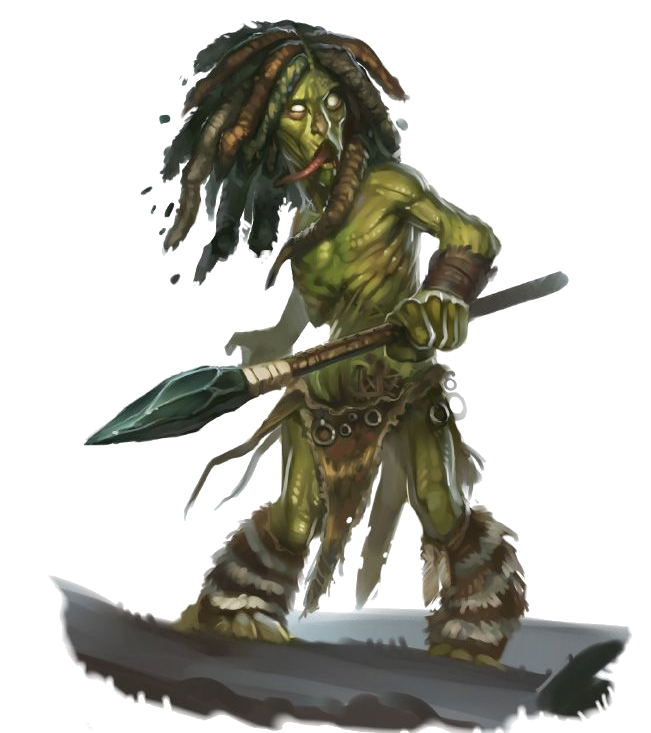
\includegraphics[width=0.48\textwidth]{02kins/img/15naenk_warrior.png}
\end{figure}

\subsection*{Naenk Names}
Naenks are born without names, and usually remain nameless most of their youth.
They reach social adulthood by earning a name, which is done either by becoming a warrior or accomplishing a major deed.

Many naenks live their whole lives unnamed.
While most accept this reality and become gatherers, it is not uncommon for the nameless to self-exile out of shame or discontent.

Knaenese is a very hard language to pronounce, so it's common for people of other kins to call naenks by a nickname or a simpler version of their name.

\paragraph{Names} Gantauda, Gesunt, Gunsedant, Hanhant, Hanseek needa, Hantadage, Huntge, Keena, Kegunseeda, Knaetseeknan, Knandage, Knudu, Kueqan, Nade, Naekuntge, Nega, Nelati, Seetun, Tsaegae, Tsege, Tsehant, Ukena.

\subsection*{Traits}
Your naenk character has an assortment of abilities, relating to their nature and surroundings.

\subparagraph{Ability Score Increase} Your Dexterity score increases by 2.

\subparagraph{Age} A naenk typically lives at most 30 years.
They are naturally mature right after being born and usually take less than a month to adapt to their society.

\subparagraph{Alignment} Naenks are organized creatures, used to following the rules of their communities.
Most tend towards the silver tide, especially those who haven't gained a name yet.

\subparagraph{Size} The moss kin come in very varied shapes and sizes.
They stand a tiny bit smaller than their birth corpse, but weight about half.
Your size and anatomy varies greatly depending on your birth corpse. \label{kin::naenk.size}

\subparagraph{Speed} Your base walking speed is 9 meters.

\subparagraph{Dual Nature} You are both humanoid and plant.

\subparagraph{Naenk armor} You gain resistance to lightning damage.

\subparagraph{Naenk claws} Because of your sharp claws, you have a base climbing speed of 6 meters.
In addition, your claws are natural weapons, which you can use to make unarmed strikes.
If you hit with them, you deal slashing damage equal to 1d4 + your Strength modifier, instead of the bludgeoning damage normal for an unarmed strike.

\subparagraph{Regeneration} As a bonus action, you can stimulate your plant cells to rapidly multiply to quickly regenerate wounds.
You regain 1 hit point, and regain 1 hit point at the start of each of your turns after, until you've restored an amount of hit points equal to twice your level.
After using this trait, you must take a long rest before using it again.
If you suffer cold, fire, or necrotic damage, this regeneration is cancelled.
Additionally, you cannot use this ability if you suffered from any of these damage types after your last turn.
You are also able to regenerate lost limbs, albeit at a very slow pace: it takes you 1d4+2 months to fully recover a lost arm or leg.

\subparagraph{Eat by Osmosis} While naenks prefer to eat meat by nature, you can mostly live off nutrients from the ground.
When in fertile land, you only need to eat once per week.
You can also eat more often if you choose to do so.

\subparagraph{Moldy Companion} Once every month, you may contaminate a recently deceased beast with nanust spores.
To do this, you must succeed on a medicine ability check of DC 8 + the number of hit dice the creature has.
If you succeed, the spores will settle into the beast, and after a week, its corpse will rise as your nuen.
The nuen has the stats, abilities, and actions of the original beast, but its hit points and hit dice are cut in half.
It also gains the Plant Camouflage ability.

If you're travelling with one or more naenks, only the naenk with the highest Wisdom score can use this trait.
If you start travelling with a naenk meeting this conditions and already have a nuen companion, it will continue following your command.

\subparagraph{Languages} You can speak, read and write Knaenese.
You can learn other languages, but your pronunciation leaves much to be desired.

% Despite their lack of lips, the moss kin does speak a language, which is named Knaenese.
% Knaenese is a very simple, accommodating to their impaired speech.
% While a naenk can learn other languages, their pronunciation usually leaves much to be desired.

\subparagraph{Subraces} Naenks are most easily separated by their home - Gannag or Na'ane.

The most common of their kin, Gannagian naenks are the members of the tribes that surround the Tekatsae tree.
They have a very strong sense of community and an excellent capacity to work as a team.
Any one naenk will easily give their life without second thought for their people and for their way of life.

While all naenks are capable fighters, Gannagian naenk take on different jobs to fulfill different tasks.
The most common of these are the warriors, the hunters, and the gatherers.
Your subrace traits depend on which of these roles you take.

\subsubsection{Gannagian Warrior}
\subparagraph{Ability Score Increase} Your Strength score increases by one.

\subparagraph{Improved Nuen} Your nuens are stronger than average, and you do not half the creature's hit points or hit dice when you raise one.
Additionally, your nuen grows a thick layer of thorns, and gains the \textbf{Natural Defense} trait (page \pageref{trait::naturaldefense}).

\subparagraph{Combat Training} Trained and proficient in combat, you know the first rank of the \textbf{Armed Fighter} talent (page \pageref{tal::armedfighter}).
Additionally, the damage die of your claws is increased from a d4 to a d6.

\subsubsection{Gannagian Hunter}
\subparagraph{Ability Score Increase} Your Constitution score increases by one.

\subparagraph{Plant Camouflage} You have advantage on Dexterity (Stealth) checks you make while in any terrain with ample obscuring plant life.

\subparagraph{Hunter's Guts} Hardened by the fiercest of the jungle, you know the first rank of the \textbf{Survivor} talent (page \pageref{tal::survivor}).
Additionally, your base climbing speed is of 9 meters instead of 6.

\subsubsection{Gannagian Gatherer}
\subparagraph{Ability Score Increase} Your Intelligence score increases by one.

\subparagraph{Darkvision} Gatherers spend most of their life recollecting fungus underground, and this provides you with an increased awareness in the dark.
You can see in dim light within 18 meters of you as if it were bright light, and in darkness as if it were dim light.
You can't discern color in darkness, only shades of gray.

\subparagraph{Seedspeech} Through simple sounds and touch, you can communicate simple ideas to living plants.
You are able to interpret their responses in simple language.
Plants do not perceive the world in terms of sight, but most can feel differences in temperature, describe things that have touched them, as well as hear vibrations that happened around them (including speech).

% A master finder, you know the first rank of the \pageref{tal::naturalist} talent (page \pageref{tal::naturalist}).
% Additionally, you can easily tell if a plant if poisonous, even if you've never encountered it before.

\subsubsection{Na'ane Naenk}
Among the naenks that grow disillusioned with their tribes, many choose to pack their possessions and leave.
Among these self-exiled naenks, most usually choose to join the neighboring nation of Na'ane to live with their tsanek brothers.

These naenks drink a special beverage upon arrival known as nahan cooked by the nations sovereigns.
% NOTE: Nahan literally means "I-water" in Knaenese.
Nahan weakens the bond of the naenk with the Tekatsae tree, forcing them to attain a qualar to remain sentient.
As a side effect, it also extends the naenk's life, pushing it to about 50 years.

\subparagraph{Ability Score Increase} You are learned the way of the tsaneks, and your Wisdom score increases by one.

\subparagraph{Rapport Spores} Your time among the tsanek has allowed your body to adapt, and fungal growths are found all around your body.
You can extend rapport spores in a 4.5 meter radius as an action.
These spores can go around corners and affect any creatures with an Intelligence score of 2 or more that aren't undead, constructs, or elementals.
Creatures affected by the spores realize the effect immediately, but those outside of range cannot notice it.
Affected creatures can communicate telepathically with one another while they remain within 9 meters of each other.
The effect lasts for 15 minutes.

\subparagraph{Noxious Spores} When a creature touches or hits you with a melee attack, you can choose to secrete noxious spores as a reaction.
The creature takes 1d6 poison damage if it isn't undead, construct, or elemental.
You can use this skill a number of times equal to your Constitution modifier (minimum of 2).
After expending your uses, you can't use this trait again until you complete a short rest.

\begin{figure}[!b]
    \centering
    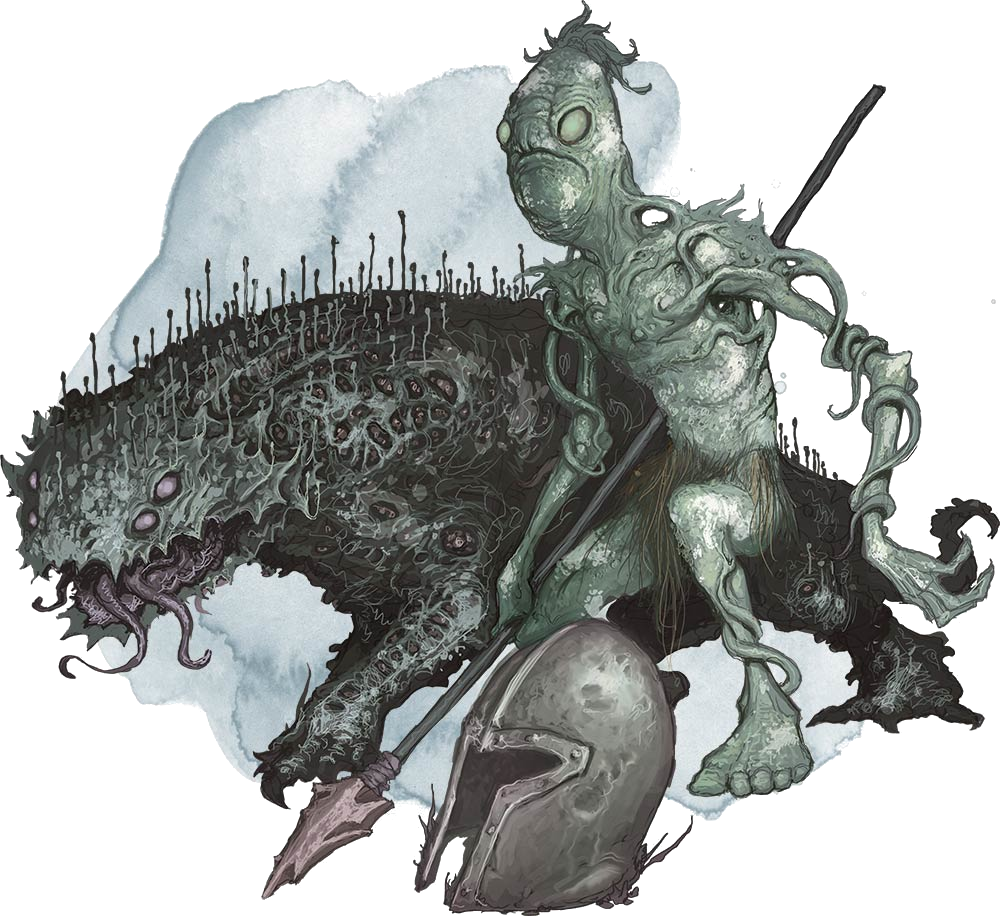
\includegraphics[width=0.48\textwidth]{02kins/img/15naenk_nuen.png}
\end{figure}
\end{linenumbers}

% % !TEX root = ../main.tex
% TODO: GENERAL CHECKUP NEEDED

\section{Fungal Kin}
\begin{linenumbers}
\DndDropCapLine{I}{ done seen some things down there.}
\textit{There be cities grander than any of gat's make, holdin' creatures stranger than the harrowing immensity isself.
There be ungodly abominations that weren't never meant to see the light o' day.
And there be... there be mushrooms! An entire city of mushrooms!}

\hspace*{\fill} --- Blim recounts their first tsanek encounter.

% TODO: MOVE TO TSANEK SECTION!

% Apart from its chief, every unit has a designated tsanek shaman.
% This tsanek is mainly in charge of communicating with the other tsaneks in faraway places, aiding in the coordination of the tribe as a whole.
% Apart from this and other ceremonial tasks, the shaman acts as a normal member of the unit.

% The highest ranking members of their society are the sovereigns and elder sovereigns, who are tsaneks that reached their final stage of development.
% The former are huge mobile tsaneks that take root in strategic positions in Drejeck to establish their complex communication network.
% The latter are the eldest in the tribe, and merge with Tekatsae itself.
% They directly speak to the tree, communicating its wishes to the sovereigns and shamans via their root network.

Also known as tsaneks in the naenk tongue, the fungal kin is a species of intelligent fungi creature that inhabit swamps, forests, and caverns.
They are commonly seen in the jungle of Drejeck, as members of the tribes near the tekatsae tree.
Like the naenks, tsaneks grow from the tree itself, starting out as small russet-colored fungi in the tree's base and exposed roots, until they're able to grow legs and emerge.
Unlike the naenks, the fungal kin are capable of reproducing by themselves, and it's very common to find independent tsanek communities in the darker reaches of Yuadrem.

Tsaneks generally deplore violence, and only attack when provoked.
If approached peacefully, they gladly provide shelter or passage through their colonies.

\subsection*{Tribal Life}
Most tsaneks belong to the tribes of Drejeck, filling the roles of shamans and diplomats that the naenks are less likely to fulfill due to their violent nature.
They are considered above their mossy companions in their social circles, and are generally treated with respect among them.

When a tsanek reaches 100 years, it is put through the rite of growth.
The tsanek must ceremoniosly consume a mixture of the sap of tekatsae, wyvernroot, and water of the boiling river. % Wyvernroot is a strong poisonous plant native to Drejeck.
Next, it must enter a chamber of awareness, which are small caverns below tekatsae.
The tsanek is only left out after a month in isolation.
Most of the tsaneks that go through this ritual die, and are consumed by tekatsae, bringing them back to the tree.
The ones that don't become the highest ranking members of their tribal societies: Sovereigns.
Tsanek sovereigns are large, malformed creatures that reign over the tribes.
They are the only creatures capable of directly speaking with tekatsae, and thus are the only that can communicate its wishes to the tribes.

\subsection*{Circles and Melds}
Many tsaneks, feeling unprepared, leave the tribes before this ritual.
Usually many more of their species follow them to start independent communities as exiles.
Over a timeframe of 300 to 400 years, the eldest from these colonies naturally grow to become sovereigns themselves, presiding over many social groups called circles.
A circle consists of twenty or more fungal kin that work, live, and meld together.

Melding is prohibited in the Drejeck tribal communities, but is a regular practice in these circles.
A meld is a form of communal meditation that allows tsaneks to transcend their sometimes dull existence.
Their rapport spores bind the participants into a group consciousness, inducing a shared dream that provides entertainment and social interaction.
Tsaneks use melding in the pursuit of higher consciousness, collective union, and spiritual apotheosis.
They can also use their rapport spores to communicate telepathically with other sentient creatures.

\subsection*{Tsanek Reproduction}
Like other fungi, tsanek reproduce by mundane sporing.
They are the only race that can retain their sentience without qualar, but if their spores grow without the influence of tekatsae or a particularly old sovereign, the sprouting quickly becomes feral, unable to retain sentience.
Due to this, tsaneks carefully control their spores' release.

Tsaneks are known to feel very little connection to their offspring.
Among the tribal tsaneks, the children of their species are taken care of by a few tsanek designated as the spore-caretakers.
Among the exiles, child rearing becomes a responsbility shared by the entire circle.
It is rare if young tsaneks can even identify their parents.

\subsection*{Call to Adventure}
While many tsanek are needed in the tribes near tekatsae for managerial tasks, it is not unusual for some to travel the globe to learn.
Most focus their study on the qualar and cter'rheth, bringing this knowledge back to their tribes.

Cavern tsaneks regularly travel the many caves below Yuadrem, and some even settle outside of their colonies, most usually in dark gat cities.
Some have founded libraries, laboratories, and monasteries, usually along oths, and dedicate their lives to research and education.

\subsection*{Tsanek Names}
Due to the fact that tsaneks have no verbal language, their names are most appropriately translated as physical descriptions of a particular individual.

\paragraph{Names} Bolete, Brownback, Buttonhead, Greenfoot, Morel, Mossy, Portabelt, Puffball, Redstem, Soft-Step, Stinkhorn, Toad.

\begin{figure}[!t]
    \centering
    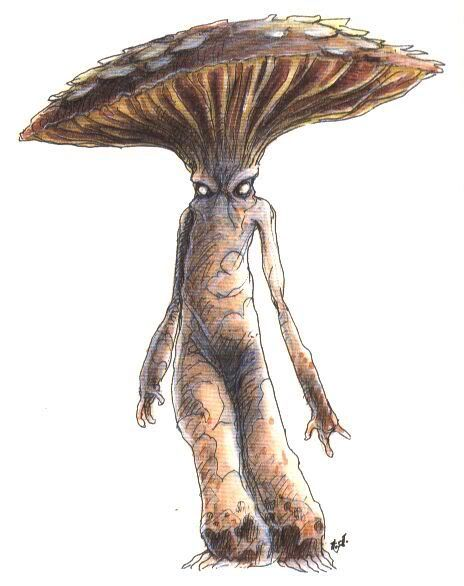
\includegraphics[width=0.48\textwidth]{03kins/img/tsanek_individual.jpg}
\end{figure}

\subsection*{Traits}
Your tsanek character has a diverse set of skills based on its nature and role on society.
\subparagraph{Ability Score Increase} Your Wisdom score increases by 1, and your Constitution score increases by 1.
\subparagraph{Size} A tsanek grows to a wide variety of heights and building, with the most common being stocky and measuring about 1.9 meters in height, and weighing around 65 kg.
Your size is medium.
\subparagraph{Speed} Your base walking speed is 9 meters.
\subparagraph{Age} Individual tsanek are not known to die of old age, and the most elder can live to become a sovereign of one or more circles, living indefinitely longer.
Sproutings take a long time to fully mature, but it's a continuous process and even the oldest tsaneks seem to continue growing, albeit slowly.
\subparagraph{Alignment} Most often, a tsanek believes strongly in society and law.
It is extremely uncommon for a tsanek to directly attack any creature that does not mean it, or its circle, harm.
Most fungal kin groups and circles dedicate their lives to knowledge, and have a tendency towards the blue tide.
\subparagraph{Darkvision} You can see in the dark within 18 meters.
You can see in dim light within the radius as if it were bright light, and in darkness as if it were dim light.
You can’t discern color in darkness, only shades of gray.
\subparagraph{Nonverbal Magic} Though you have no conventional language, you can ignore the verbal component of spells.
\subparagraph{Rapport Spores} All creatures within 4.5 meters of you with an Intelligence score of 2 or higher that aren't undead, constructs, or elementals can communicate telepathically with you and with each other.
You can suppress this ability at will.
Creatures affected by the spores realize the effect immediately, but those outside of range cannot notice them.
Affected creatures can communicate telepathically with one another while they remain within 9 meters of each other.
\subparagraph{Pacifying Spores} As an action, you can eject spores at one creature you can see within 1.5 meters of you.
The target must succeed on a Constitution saving throw or be stunned for 1 minute.
The spell save DC for this effect is 10 + your Constitution modifier.
Undead, constructs, and elementals automatically succeed on this save.
The target can repeat the saving throw at the end of each of its turns, ending the effect on itself on a success.
After using this trait, you cannot do so again until you finish a short rest.
\subparagraph{Hallucination Spores} As an action, you can produce spores that affect all creatures within 9 meters of you that aren't undead, constructs, or elementals.
These creatures are all affected as per the cantrip minor illusion while you concentrate on the effect.
The spell save DC is 10 + your Constitution modifier.
\subparagraph{Languages} You can understand, read and write naenk tongue and one other language of your choice, but you cannot speak.

\begin{table*}[b]%
    \begin{DndTable}[width=\linewidth]{X}
        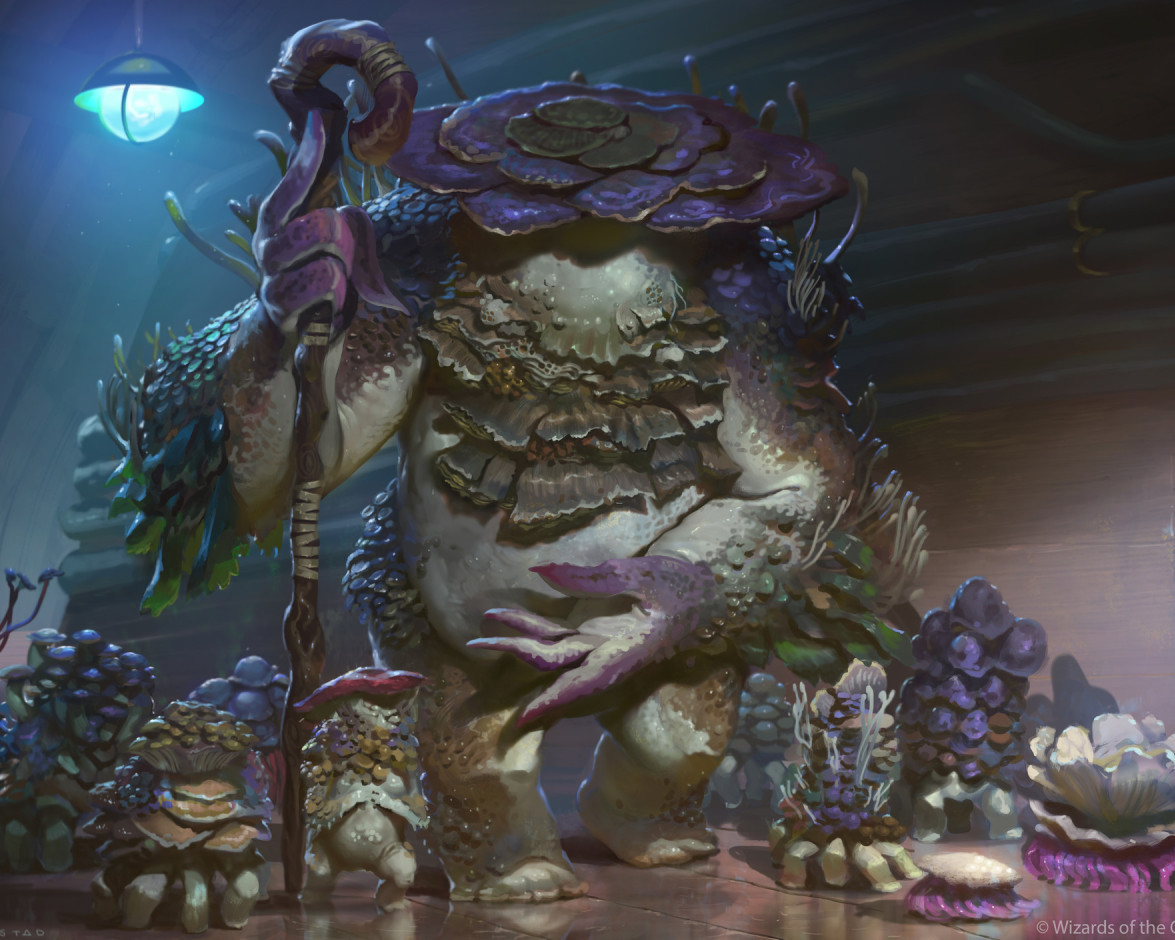
\includegraphics[width=0.98\textwidth]{03kins/img/tsanek_sovereign.jpg}
    \end{DndTable}
\end{table*}

\subsubsection{Ke'ena Tsanek}
Fungal kin that are members of the tribes in Drejeck which surround tekatsae.
Like their mold kin brothers, they have a very strong sense of community and devotion to their groups, the sovereigns and the tekatsae tree.
They are the spiritual leaders of the different groups, and focus on coordinating the tribes and communicating with the sovereigns.
\subparagraph{Ability Score Increase} You focused much of life in study, and your Wisdom score increases by 1.
\subparagraph{Drug-enhanced Spores} Your Rapport Spores range is increased to 9 meters, and the spell save DC of both your Pacifying Spores and Hallucination Spores changes to 8 + your Constitution modifier + your proficiency bonus.
\subparagraph{Euphoria Spores} Accustomed to fighting with the naenk warriors, you can release a specialized cloud of spores in a 6-meter-radius sphere centered on yourself.
Other creatures in that area must make a Constitution saving throw of a DC equal to 8 + your Constitution modifier + your proficiency bonus or become poisoned for 1 minute.
A creature can repeat this saving throw at the end of each of its turns, ending the effect early on itself on a success.
When the effect ends, the creature gains one level of exhaustion.
You can produce these spores a number of times equal to your Constitution modifier (minimum of 2) per long rest.

\subsubsection{Cavern Tsanek}
Sometimes, a tsanek will decide to abandon the tribe and break its link with the tekatsae tree.
These tsanek, unable to forgo their community lifestyles, tend to join or form fungus kin communities in the caverns of the world, sometimes spawning huge underground fungus cities.
\subparagraph{Ability Score Increase} Your meandering in hostile environments has granted you increased resilience, and your Constitution score is increased by 1.
\subparagraph{Sun Sickness} You become poisoned if you spend more than 1 minute in direct, unobstructed sunlight.
This conditions ends when you spend 1 minute in dim or dark conditions.
\subparagraph{Superior Darkvision} Accustomed to the darkness of the deepest caverns, you have superior vision in dark and dim conditions.
You can see in dim light within 36 meters of you as if it were bright light, and in darkness as if it were dim light.
\subparagraph{Meld} When you take a short or long rest in the presence of two or more other tsaneks, you can meld with them.
After melding, you regain all expended Hit Dice and gain the following benefits:
\begin{itemize}
    \item You have advantage on a saving throw you make in the next 24 hours.
    \item You can end one disease or condition affecting you, be it blinded, deafened, paralyzed, or poisoned.
\end{itemize}
\subparagraph{Communal Intellect} Your time spent melding with the others of your kin has granted you a deeper understanding of the world and yourself.
You are proficient in the Insight skill, and you have advantage on Wisdom (survival) checks made to find your way in caverns.
\end{linenumbers}

% % TODO: GENERAL CHECKUP NEEDED

\section{Shelled Kin}
\begin{linenumbers}
\textit{I caught a big fish.}

\textit{Now I search for a good friend}

\textit{To share my lunch with.}

\hspace*{\fill} --- Tortle haiku.

The shelled kin are a species native to the outer lands.
Also known as tortles, they have gracefully adapted to their lives in Yuadrem, able to start a new life in the land ravaged by the schism, and it is very common to see the rustic tortle villages in the coasts of the beryl sea and many of the eastern shores of the continent.
% The shelled kin or tortles are a species native to the outer lands which, unlike umans, don't seem to be hunted by the strange creatures from this place, and remain unaffected by the forbidden lands.

What many tortles consider a simple life, others might call a life of adventure.
Tortles are born near sandy coastlines, but as soon as they're able to walk on two legs, they turn into nomad survivalists eager to explore the wilderness, experience its many wonders, put their skills to the test, and make new acquaintances.

\begin{figure}[!b]
    \centering
    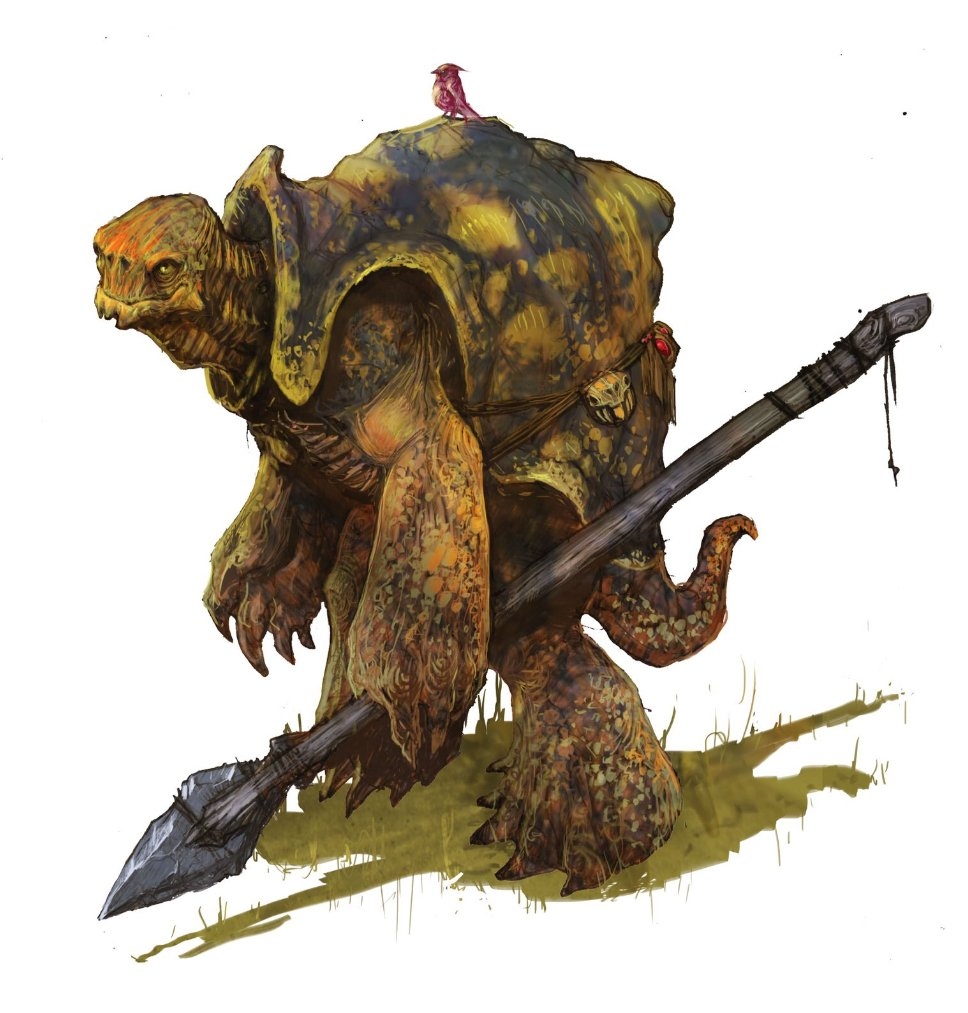
\includegraphics[width=0.48\textwidth]{03kins/img/tortle_official.jpg}
\end{figure}

\subsection*{Life of a Tortle}
A tortle hatches from a thick-shelled egg and spends the first few weeks of its life crawling on all fours.
Its parents usually leave soon after its birth, but spend what little time they have telling stories to their offspring. 
Within a year, the young tortle is abandoned and becomes an orphan, though not before it learns to speak and to survive on its own.

A young tortle and its siblings inherit whatever tools, weapons, and gifts their parents leave for them.
Each young tortle is expected to fend for itself.
It leaves the place of its birth and finds its own corner of the wilderness in which to hunt, catch fish, and get by.
With each passing year, a tortle hones its survival skills.
It forms friendships with its neighbors while also respecting their privacy.
At some point, a tortle feels an almost overwhelming urge to venture far away from home and see more of the world.
It gathers up its possessions and heads into the wilderness, returning months or years later with stories of its exploits and new skills.

Tortles are gendered creatures, and it is usual for them to seek out a mate and procreate when they return home from these travels.
Tortles lay their eggs (numbering as few as one or as many as a dozen) in a fortified compound enclosed by stone walls that are easily defensible.
If no such compound exists, they build one.
The parents spend the hatching time of their eggs guarding the compound and defending their offspring, and after they hatch they spend a year sharing their knowledge with the young ones.
The parents leave their children at this time, overburdened by their nomadic nature and confident that the older tortles of the village will care for them.
When the children are old enough to leave the compound, they pick up whatever weapons and tools their parents left behind and set out on their own.

\subsection*{Beliefs}
Tortles don't have a religion of their own, but they often worship the gods of other races.
It's not unusual for a tortle to hear stories or legends related to a god and choose to worship that deity.
Curious in nature, most tortles like to see how other creatures live and discover new customs and new ways of doing things.
Some tortles are also drawn to the many schools of thought, trying to learn from all of them instead of focusing on a single one.

Tortles believe that night and day watch over them and other creatures.
The moons are the eyes of night that watch over them in darkness, and the sun is the equally vigilant eye of day.
Tortles feel most at peace when these "eyes" are looking down on them.
They become more nervous and uneasy when no orb is visible in the sky.
Tortles tend to be most uncomfortable underground, where neither the sun nor the moons are visible to them.

Blessed are the days when many moons are visible in the sky at the same time.
Tortles often choose such days to leave their homes and begin a wilderness expedition, or perform some other task they know to be dangerous.

\subsection*{Inherent Mutualism}
Tortles have a special relationship to the anchelons.
Anchelons are colossal horned turtles that reside in Yuadrem's oceans, breeding fear among sailors and fishers alike.
They are generally fierce in nature but, while not sentient, they are oddly friendly toward tortles.
Anchelons lay their eggs in the beryl sea, and tortles allow thme to lay their eggs in their compounds.
It is not uncommon for baby anchelons to grow alongside tortles.
Anchelons in exchange protect the tortles' villages, and may even help tortles they encounter in the wilds.

\subsection*{Adventurers at Heart}
Tortles have a saying: "We wear our homes on our backs."
The shells they carry around provide all the shelter they require.
Consequently, tortles don't feel the need to root themselves in one place for too long.
A tortle settlement is primarily used as a kind of moot, where tortles can socialize with one another, share useful information, and trade with strangers in the safety of greater numbers.
Tortles don't regard these settlements as places worth defending with their lives, and they will abandon a settlement when it no longer serves their needs.

Tortles embrace a simple view of the world.
It is a place of wonder, and tortles see beauty in the ordinary.
They live for the chance to hear a soft wind blowing through palm trees, to watch a frog croaking on a lily pad, or to stand in a crowded marketplace.

Tortles like to learn new skills.
They craft their own tools and weapons, and they are good at building structures and fortifications.
They marvel at the works of other kins, and can lose themselves for years in a city, studying its architectural wonders and learning skills they can put to use when building forts to contain their offspring.

Although they spend a considerable portion of their lives in isolation, tortles are social creatures that like to form meaningful friendships.
Being native to another world, they have no inbred animus toward any kin.
In fact, a tortle will often seek out friendships with non-tortles to learn new customs and new points of view.

% \begin{figure}[!htbp]
%     \centering
%     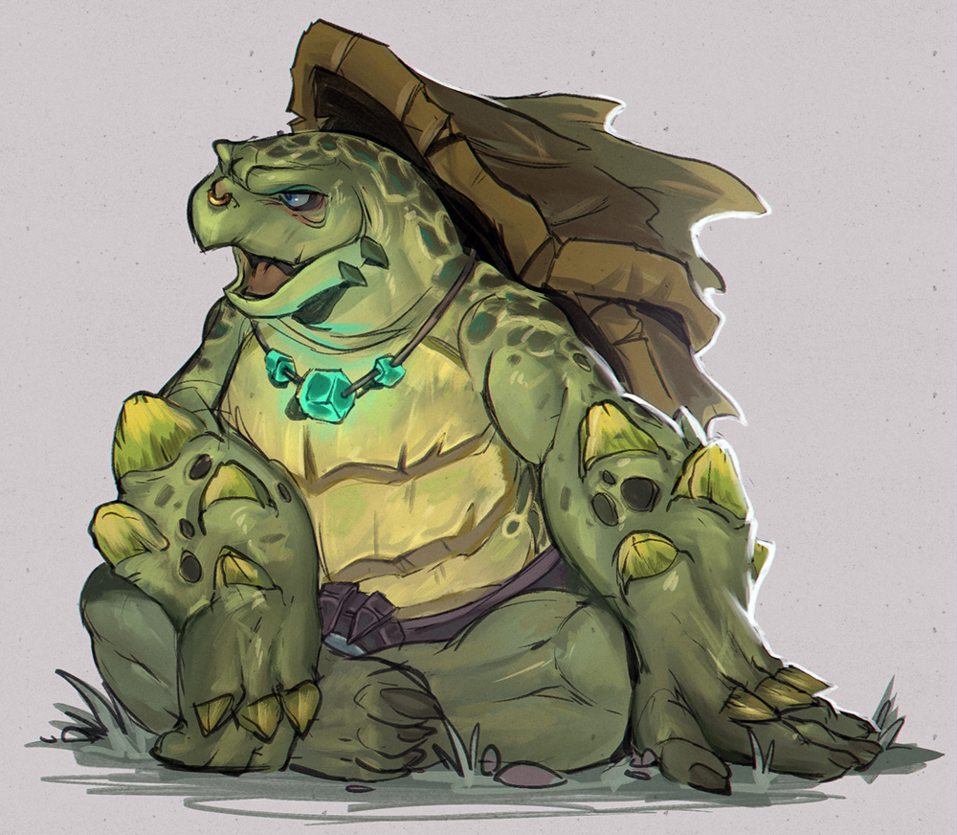
\includegraphics[width=0.48\textwidth]{03kins/img/tortle_chill.png}
% \end{figure}

\subsection*{Tortle Names}
Tortles prefer simple, non-gender-specific names that are usually no more than two syllables long.
If a tortle doesn't like its name for whatever reason, it can change it, and it might do this a dozen times in its life.

A tortle doesn't feel constrained by its name, which is designated only to refer to the tortle in contrast of its peers.
Tortles don't have surnames or family names.

\paragraph{Names}
Baka, Damu, Gar, Gura, Ini, Jappa, Kinlek, Krull, Lim, Lop, Nortle, Nulka, Olo, Ploqwat, Quee, Queg, Quott, Sunny, Tibor, Ubo, Uhok, Wabu, Xelbuk, Xopa, Yog

\subsection*{Traits}
Your tortle character gains traits that enable it to cope with the perils of a savage world.
\subparagraph{Ability Score Increase} Your Strength score increases by 2, and your Wisdom score increases by 1.
\subparagraph{Age} Young tortles crawl for a few weeks after birth before learning to walk on two legs. 
They reach adulthood by the age of 15 and live an average of 500 years.
\subparagraph{Alignment} Tortles tend to lead orderly, ritualistic lives.
They develop customs and routines, becoming more set in their ways as they age.
Most follow a set of tenets that the kin brought with them from the outer lands, leading to lawfulness.
While most are good, a few can be selfish and greedy, but it's unusual for a tortle to shuck off order in favor of chaos.
Tortles tend towards the gold tide, always empathic and helping others.
\subparagraph{Size} Tortle adults stand 1.5 to 1.8 meters tall and average 230 kg.
Their shells account for roughly one-third of their weight.
Your size is Medium.
\subparagraph{Claws} Your claws are natural weapons, which you can use to make unarmed strikes.
If you hit with them, you deal slashing damage equal to 1d4 + your Strength modifier, instead of bludgeoning damage normal for an unarmed strike.
\subparagraph{Hold Breath} Tortles aren't natural swimmers, but they can remain underwater for some time before needing to come up for air.
You can hold your breath for up to 1 hour at a time.
\subparagraph{Natural Armor} Due to your shell and the shape of your body, you are ill-suited to wearing armor.
Your shell provides ample protection, however; it gives you a base AC of 17 (your Dexterity modifier doesn't affect this number).
You gain no benefit from wearing armor, but if you are using a shield, you can apply the shield's bonus as normal.
\subparagraph{Shell Defense} You can withdraw into your shell as an action.
Until you emerge, you gain a +4 bonus to AC, and you have advantage on Strength and Constitution saving throws.
While in your shell, you are prone, your speed is 0 and can't increase, you have disadvantage on Dexterity saving throws, you can't take reactions, and the only action you can take is a bonus action to emerge from your shell.
\subparagraph{Survival Instinct} You gain proficiency in the Survival skill.
Tortles have finely honed survival instincts.
\subparagraph{Learned Tradition} You are proficient with two weapons, two sets of artisan's tools, or one of each of your choice.
This comes from the time spent with your parents, and you feel a special connection with these types of items.
\subparagraph{Languages} You can speak the krehlo tongue and one additional language of your choice, but cannot write or read either.
The krehlo tongue doesn't have a written form, and the tortle tenets are passed on in oral tradition.

\begin{table*}[b]%
    \begin{DndTable}[width=\linewidth]{X}
        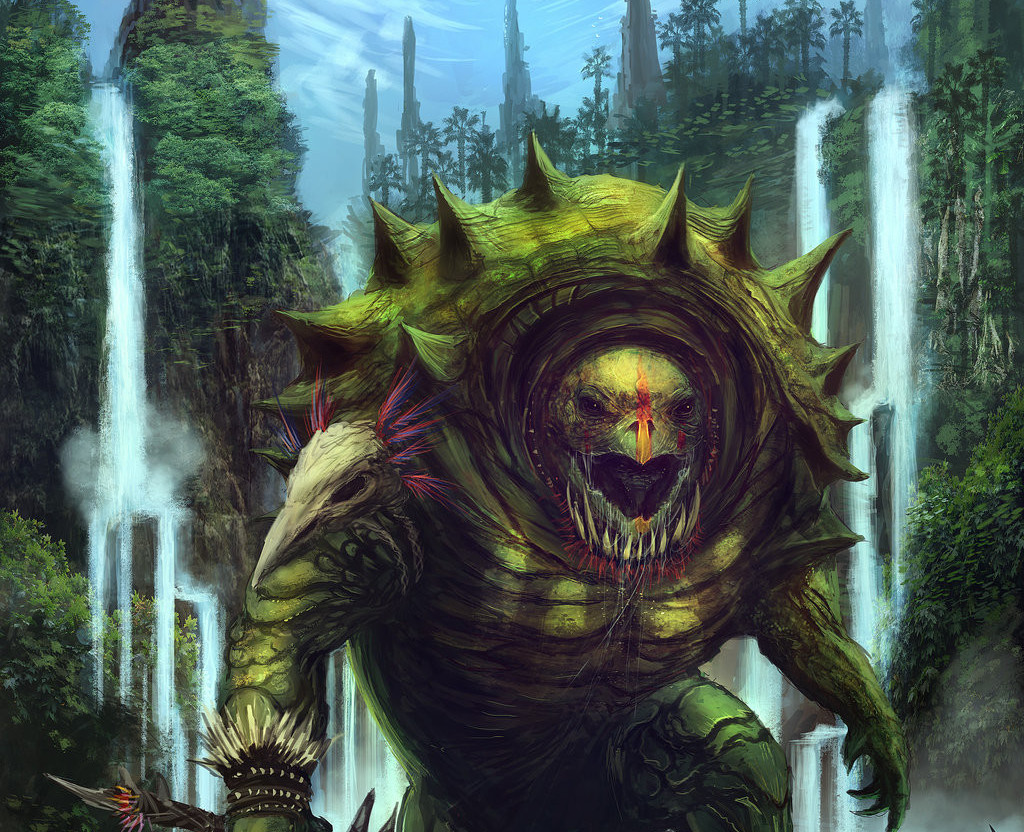
\includegraphics[width=0.98\textwidth]{03kins/img/tortle_spiked.jpg}
    \end{DndTable}
\end{table*}

\subsubsection{Steam Kin}
A very small proportion of the shelled kin population are born with special characteristics.
Their bodies are slightly larger and are of a stony appearance and color, their teeth are larger and sharper, and they have small growths on the top of their heads resembling tiny horns.
Their larger bodies prohibit them from nesting inside their shells.
They make up this lack of defense with a stronger offense however.
\subparagraph{Size} The steam kin are larger in nature than the average tortle.
Adults stand between 180 and 200 cm, and weigh on average 280 kg.
\subparagraph{Steam Breath} This trait replaces shell defense.
You can use your action to exhale a 20 feet cone of scalding steam.
Every target in the area must make a Dexterity saving throw, with a DC of (8 + your Constitution modifier + your proficiency bonus).
A creature takes 2d6 fire damage on a failed save, or half as much damage on a successful one.
The fire damage increases to 3d6 at 6th level, 4d6 at 11th level, and 5d6 at 16th level.
After you use this trait, you can't use it again until you complete a short or long rest.
Being underwater doesn't grant resistance to this damage.
\end{linenumbers}

\begin{DndSidebar}[float=!b]{Variant Tortle Trait}
    Being born of the communion of two beings, tortles present slight genetic differences based on their family trees.
    Tortles born in the settlements near Leeside possess one such difference, and are known to be born with a spiked shell.
    You can choose to replace your claws trait with impaling carapace.
    \subparagraph{Impaling Carapace} When you grapple a creature, the target takes 1d4 piercing damage if your grapple check succeeds.
    If another creature grapples you, they take 1d4 piercing damage.
    If you start your turn grappling or being grappled by a creature, it takes 1d4 piercing damage.
\end{DndSidebar}

% % !TEX root = ../main.tex
% TODO: GENERAL CHECKUP NEEDED

\section{Poison Kin}
\begin{linenumbers}
\DndDropCapLine{T}{hey're a poison spilled down onto}
\textit{ our world, I tell ya'!
Grungs're bad.
They real bad!
They tell ya' their skin be the worst part o'em, but they don't know!
The spears mon.
It's the spears!}

\hspace*{\fill} --- Kleeck recounts her brief visit to Mabela.

Also known as grungs, the poison kin are aggressive creatures that look similar to dart frogs.
The species quickly settled into the chirping wilds and the areas surrounding the rainforest after their arrival during the schism.
They are fiercely territorial and see themselves as superior to most other creatures.

\subsection*{Class Structure}
Grung society is a caste system.
Each caste lays eggs in a separate hatching pool, and juvenile grungs join their caste upon emergence from their hatchery.
All grungs are a dull greenish gray when they are born, but each individual takes on the color of its caste as it grows to adulthood.
From lowest to highest caste, grungs are green, blue, purple, red, orange, and gold.

Green grungs are the tribe's warriors, hunters, and laborers, and blue grungs work as artisans and in other domestic roles.
Supervising and guiding both groups are the purple grungs, which serve as administrators and commanders.
Red grungs are the tribe's scholars and sorcerers.
They are superior to purple, blue, and green grungs and given proper respect even by the grungs of higher status.
Higher castes include orange grungs, which are elite warriors that have authority over all lesser grungs, and gold grungs, which hold the highest leadership positions.
A tribe's sovereign is always a gold grung.

A grung normally remains in its caste for life.
On rare occasions, an individual that distinguishes itself with great deeds can earn an invitation to join a higher caste.
A mixture of godsblood, seawater and poison is blessed by a red grung, and by drinking it the elevated grung changes color and is inducted into its new caste in the same way that a juvenile of the caste would be.
From then on, the grung and its progeny are members of the higher caste.

\subsection*{Poisonous Skin}
All grungs secrete a substance that is harmless to them but poisonous to other creatures.
A grung can also use this secretion as venom to coat its weapons.
Grungs are always on the lookout for creatures they can capture and enslave, and use slaves for all manner of menial tasks and hard labor.
Slaves are fed mildly poisoned food to keep them lethargic and compliant.
A creature afflicted in this way over a long period of time becomes a shell of its former self, and it seldom can be restored to normalcy.
Being amphibious, grungs require water to live; any grung that fails to immerse itself in water for at least 1 hour during a day becomes quite exhausted.

\subsection*{Whistle Stick}
All grungs are trained to use a musical instrument called the whistle-stick.
This is a hollow wooden tube with holes cut throughout, much like a flute.
Grungs play music with it for entertainment, but can also swing it about by a sturdy cord to create a sound recognizable by others of their kin, so they know each other's approximate location.
Additionally, any creature that can speak the krehlo language can use a whistle stick in this manner to communicate over distance.

\subsection*{Outcast or Voyager}
Since social advancement among grungs can only be achieved by a great deed, it is not unusual for a grung or a small group of them to travel around the coasts and rivers of Yuadrem.
They attempt to obtain renown by murdering an enemy of their civilization, or by bringing a rare artifact or important strategic information.

While a rare occurrence, sometimes an individual grung or even entire family-lines can grow disillusioned by the hardships of class advancements.
Some of them decide to escape from their cities, leading lives of their own as independent colonies or as members of the rare cities or towns willing to accept them.
Individuals from these groups are known to follow a life of adventure to help their communities or simply to satiate an internal need for excitement in the grung's heart.

\subsection*{Grung Names}
Grungs usually have simple, non-gender-specific names with a strong consonant joined by a syllable with a glottal stop, but members of higher castes prefer longer, more elaborate names to reflect their status.
Their names don't actually come from the krelho language, but are made based on what's easier to pronounce for the grung.
Grungs also wear their city of origin as surname.

\paragraph{Names}
B'ang, B'leep, B'lip, B'loop, Bl'eg, Bl'myeek, Bl'ngiip, Ch'eg, Ch'rol, D'aht, D'khan, F'huu, Fl'aak, Fl'uup, G'lahp, Gh'rol, K'eet, K'riig, K'ung, R'ang, R'loo.

\paragraph{Surnames} Bakagar, Bomqueeg, Gor, Int, Joppank, Kangaru, Limlim, Mabela, Obu, Om, Ploqlek, Queequio, Quott'nem, Uhok'moa, Wewat, Xilkoko, Zipqueg.

\begin{figure}[!t]
    \centering
    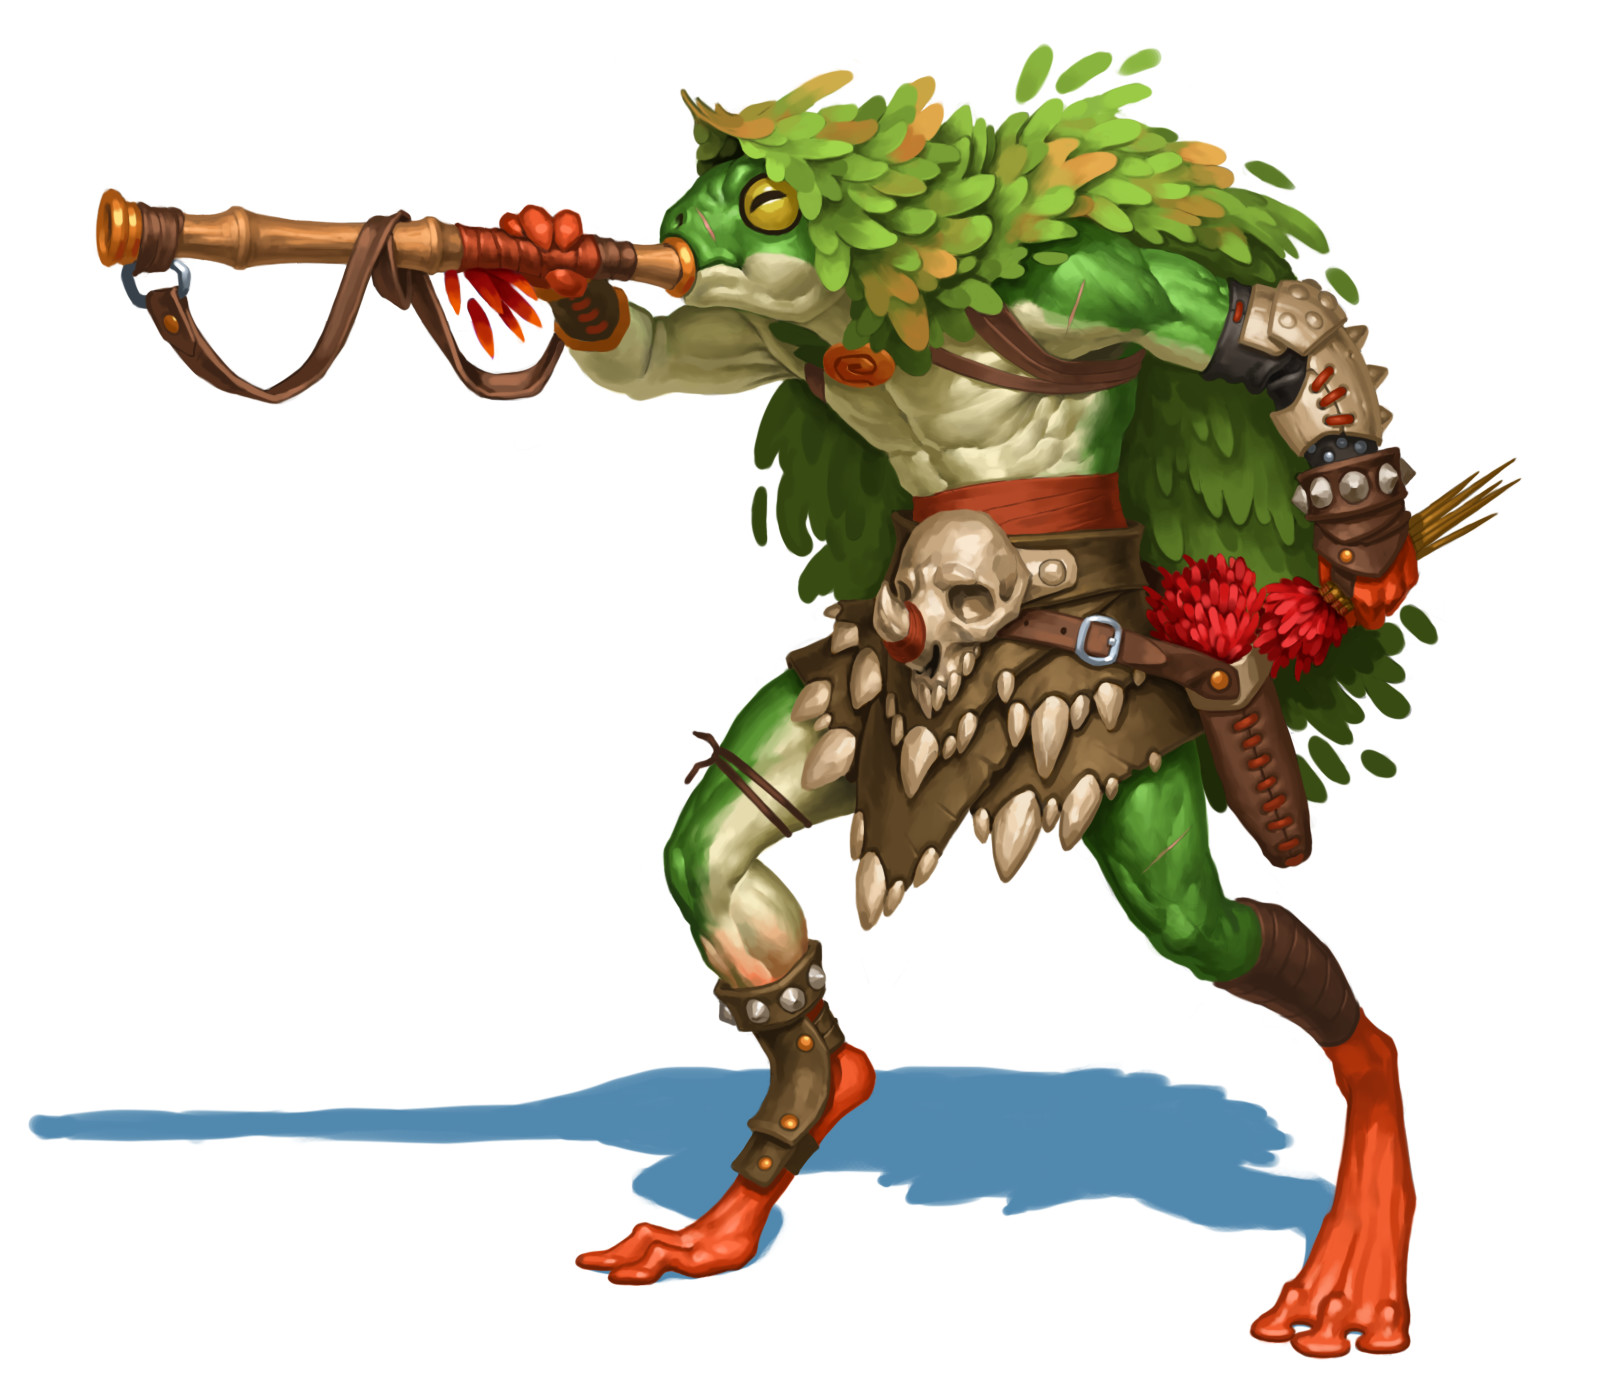
\includegraphics[width=0.48\textwidth]{02kins/img/18grung_blowgun.jpg}
\end{figure}

\subsection*{Traits}
Your grung character has an assortment of inborn abilities, part and parcel of grung nature:
\subparagraph{Ability Score Increase} Your Dexterity score increases by 2, and your Constitution score increases by 1.
\subparagraph{Age} Grung reach adulthood in a single year, and can live for up to 80 years.
\subparagraph{Alignment} % Most grungs are lawful, having been raised in a strict caste system.
% Grung society is in constant search of power, and most individual grung look forward to very rare social advancement.
Grungs are in constant search of power, and move along the silver tide.
\subparagraph{Size} Grungs stand between 75 and 105 cm tall and average about 20 kg.
Your size is small.
\subparagraph{Speed} Your base walking speed is 7.5 meters, and you have a climbing speed of 7.5 meters.
\subparagraph{Arboreal Alertness} You have proficiency in the Perception skill.
\subparagraph{Amphibious} You can breathe both air and water.
\subparagraph{Poison Immunity} You are immune to poison damage and the poisoned condition.
\subparagraph{Poisonous Skin} Any creature that grapples you or otherwise comes into direct contact with your skin must succeed on a Constitution saving throw of DC 10 + your Consitution modifier, and become poisoned for 1 minute on a fail.
A poisoned creature no longer in direct contact with you can repeat the saving throw at the end of each of its turns, ending the effect on a success.

You can also apply this poison to any piercing weapon as part of an attack with that weapon. % though when you hit the poison reacts differently.
The target must succeed on the same saving throw or take 2d4 poison damage.
A grung succeeds on these saving throws automatically.

A creature poisoned by a grung suffers an additional effect that varies depending on the grung's skin color.
This effect lasts for one turn and can only be used once per short rest.

\paragraph{Green Toxins} The poisoned creature can't move except to climb or make standing jumps.
If the creature is flying, it can't take any actions or reactions unless it lands.
\paragraph{Blue Toxins} The poisoned creature must shout loudly or otherwise make a loud noise at the start and end of its turns.
\paragraph{Purple Toxins} The poisoned creature feels a desperate need to soak itself in liquid or mud.
It can't take actions or move except to do so or to reach a body of liquid or mud, unless no such body can be found in a 90 meter radius.
\paragraph{Red Toxins} The poisoned creature feels extreme hunger and must use its action to eat something or to move towards a source of food, unless no source of food can be found in a 90 meter radius.
\paragraph{Orange Toxins} The poisoned creature becomes frightened of its allies.
\paragraph{Gold Toxins} The poisoned creature is charmed and permanently learns how to speak basic krehlo.

\subparagraph{Standing Leap} Your long jump is up to 7.5 meters and your high jump is up to 4.5 meters, with or without a running start.
\subparagraph{Grung Weapon Training} Due to combat training, you are proficient with spears, blowguns, and nets.
\subparagraph{Inflatable Cheek Pouches} Due to your frog-like anatomy, you are able to shoot darts at incredible speed.
You can shoot darts with a blowgun to a range of 15/30 meters, and the weapon's damage die is increased to 1d4.
\subparagraph{Water Dependency} If you fail to immerse yourself in water for at least 1 hour during a day, you suffer one level of exhaustion at the end of that day.
You can only recover from this exhaustion by immersing yourself in water for at least 1 hour.
\subparagraph{Languages} You can speak the krehlo tongue and one additional language of your choice, but cannot write or read either.

\begin{figure}[!b]
    \centering
    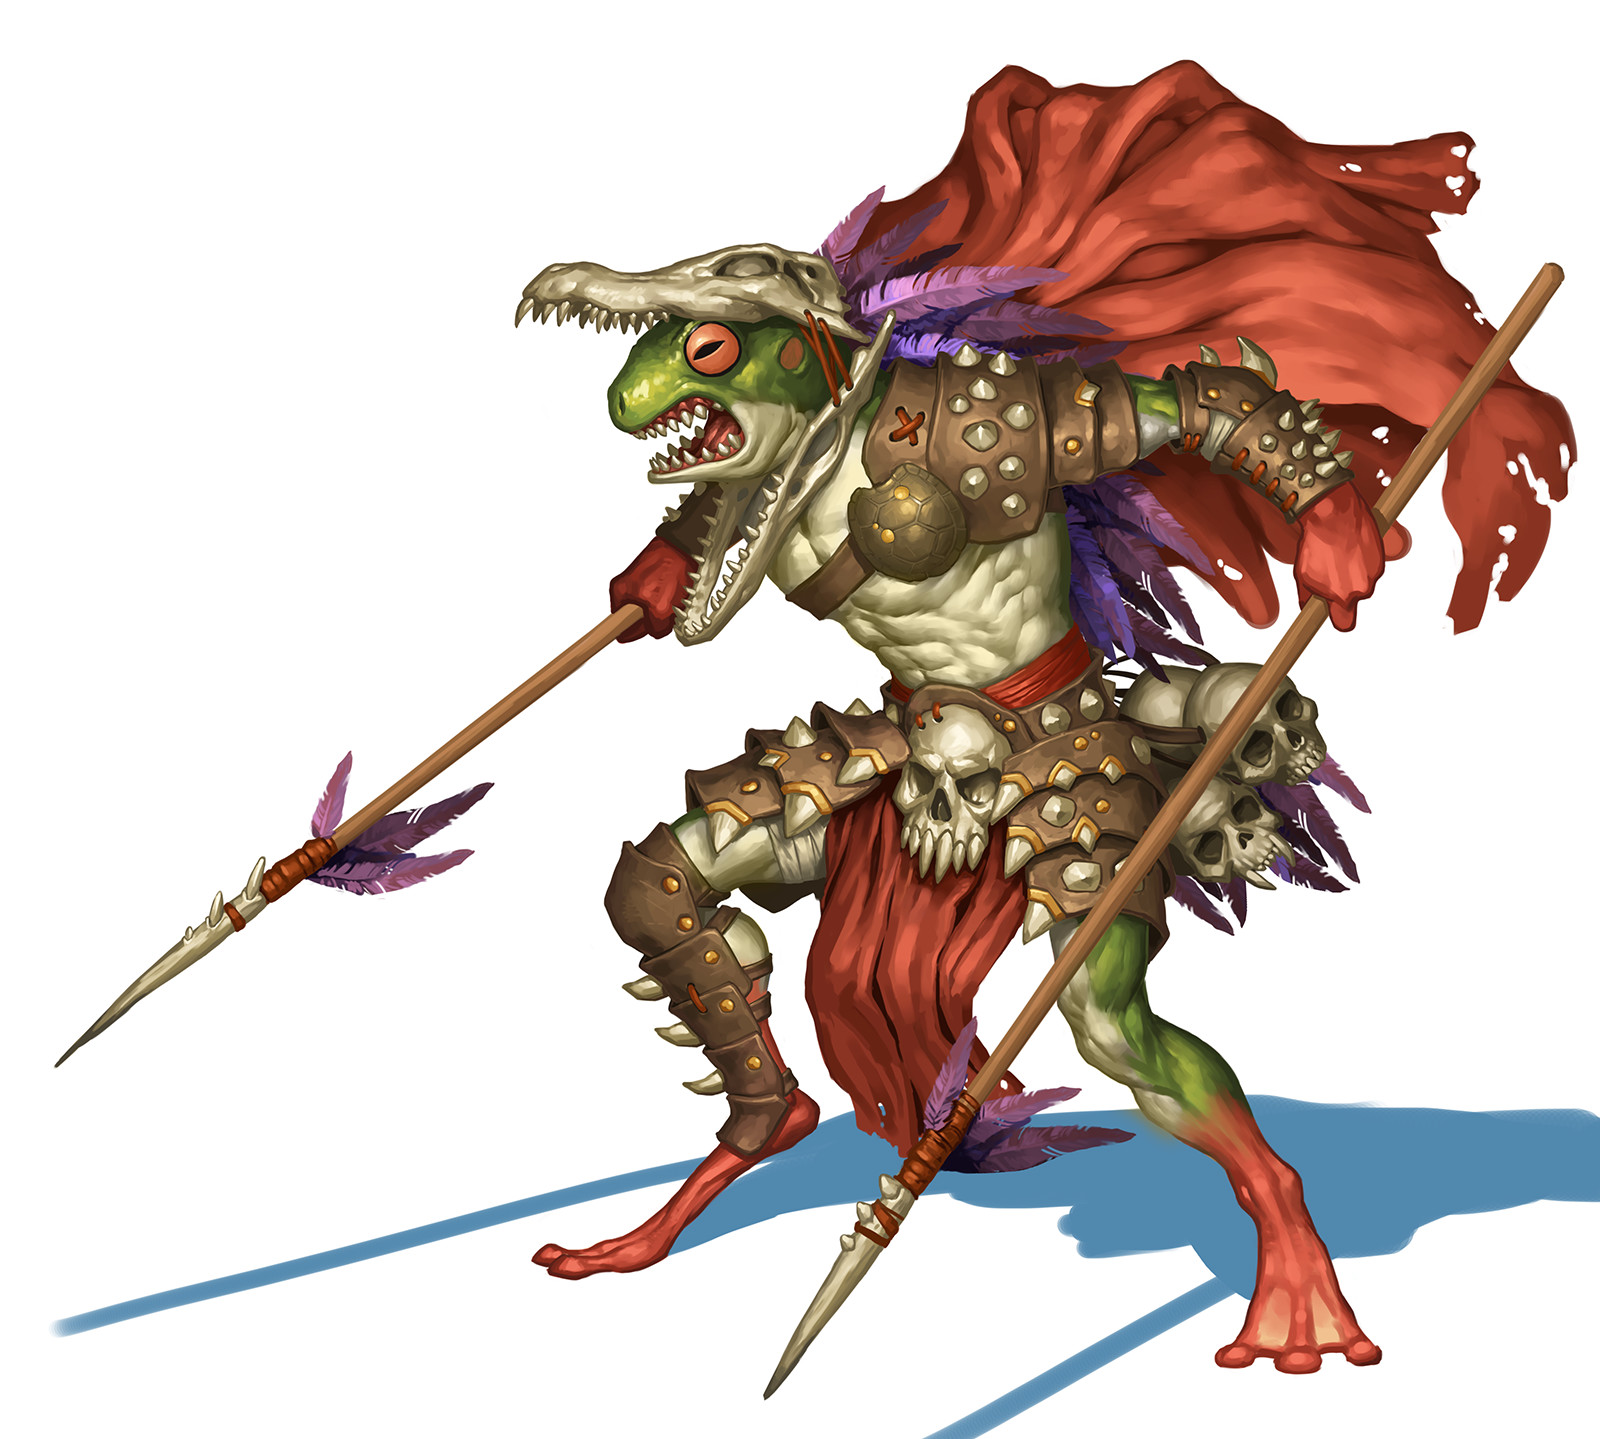
\includegraphics[width=0.48\textwidth]{02kins/img/18grung_warrior.jpg}
\end{figure}
\end{linenumbers}

% % !TEX root = ../main.tex
% TODO: GENERAL CHECKUP NEEDED

\section{Nomad Kin}
\begin{linenumbers}
\DndDropCapLine{O}{utsiders, the lot of them. Dragged}
\textit{into our world by an unnatural pull, ever unable to find stable footing.
No matter how much they beg and cry, do not allow them into your home.
Touched by a strange flame, whose brightness attracts equally as strange beasts into your door, into your hearth.
Get rid of them before they share their misfortune with you.}

\hspace*{\fill} --- Abneh, renowned nimrod.

Brought into this world with the Schism, the nomad kin are a strange race from the outer lands.
Also known as umans, they have almost hairless bodies, and are similar in appearance to apes.

For an unknown reason, umans attract all kinds of predators from these lands.
Additionally, their blood has similar properties to the tall ones', and is used in many rituals.
Because of these reasons, umans are dispersed all around the world, and are nomadic in nature.

\subsection*{A Broad Spectrum}
Hunted by all kinds of kin and creatures, the nomad kin are forced to perpetually migrate and adapt to different environments, making them more physically diverse than the common kins.

There is no typical uman, with an individual standing from 1.5 meters to a little over 1.8 meters tall, and weighing from 60 to 125 kgs.
Acclimating to even the most extreme environments, a uman's skin shades to any color from the darkest brown to the lightest hues.
They also grow long hair in their scalps and faces, sporting a great variety of colors and thickness.
Nomads reach adulthood at around 14, and rarely live a single century.

Umans are a gendered kin, and usually have one child at a time.
Families consist of a father, a mother, and their kid or children, but it is not uncommon for other members of the nomadic groups to care for parentless children.

\subsection*{Accursed Coldblood}
Known as coldblood due to its cerulean tint, Umans' blood has special properties, and is very useful for spellcasters.
It retains a sort of energy, and can be used as a source of spells.
Umans know this, and regularly prepare blood vials for trade and to strengthen troupes' wizards.

Umans pay dearly for this special blood, as it acts as a beacon for the predators from the outer lands, the coldblood beasts.
These creatures hunt umans, and many of the kin are banned from villages for safety concerns.

Spellcasters seek coldblood, and many try to attain it by any means available.
Naturally, the murder of umans for their blood is illegal in most nations, but some carry the custom on nevertheless.
The nimrods are a cult that specializes in gathering coldblood via any means available, and are commonly contracted by wizards and warlocks to attain the product.

\subsection*{Adaptable and Durable}
Hunted by both beast and kin, umans have trouble trusting others and don't normally settle in communities of other kins.
They live in troupes exclusive to their kin, where usually all members have some familiar relationship.
Troupes travel together and care for each other, assigning specific roles to each member based on their skills.

Far from vulnerable, most troupes are fierce and resilient, hardened by centuries of being preyed upon.
Groups keep track of how they are treated by different cities and towns, and only do commerce where they are accepted.

While uncommon, some uman communities have managed to settle in one place.
These communities keep their locations secret, communicating it only to other umans via traveller's cant, a set of writings and symbols they brought from the outer lands.

\subsection*{Life in Escapade}
For a uman, a life of adventure is not a romantic desire but rather a fact of mundane life.
Used to the hardships of survival, a uman is especially capable of fending off threats and surpassing hardships.

It is very common to see lone uman adventurers, either as exiles or in a quest for their troupe.
Whatever the motive, they naturally excel at voyages, and are a great fit on any adventuring party.

\subsection*{Uman Names}
Umans most commonly wear names from other cultures.
Even in the outer lands, umans were known to have a great variety of names depending on each specific culture.
Those who desire to conserve their roots choose old names from their history and legends to give their children.

\paragraph{Common Names}
(Male) Anton, Aseir, Diero, Dorn, Evendur, Grim, Haseid, Ivor, Khemed, Kosef, Marcon, Morn, Pavel, Pieron, Rimardo, Romero, Salazar, Sergor, Umbero, Zasheir;
(female) Atala, Arveene, Balama, Ceidil, Chessail, Dona, Faila, Jasmal, Luisa, Lureene, Marta, Quara, Rowan, Seipora, Selise, Shandri, Vonda;
(surnames) Agosto, Amblecrown, Astorio, Basha, Buckman, Calabra, Domine, Evenwood, Falone, Greycastle, Khalid, Kulenov, Marivaldi, Marsk, Nemetsk, Pashar, Pisacar, Ramondo, Rein, Starag.

\paragraph{Frostburn Names}
(Male) Ander, Blath, Bran, Frath, Geth, Lander, Luth, Malcer, Stor, Taman, Urth;
(female) Amafrey, Betha, Cefrey, Kethra, Mara, Olga, Silifrey, Westra;
(surnames) Brightwood, Helder, Hornraven, Lackman, Stormwind, Windrivver.

\paragraph{Boggart Names}
(Male) Aoth, Bareris, Ehput-Ki, Kethoth, Mumed, Ramas, So-Kehur, Thazar-De, Urhur;
(female) Arizima, Chathi, Nephis, Nulara, Murithi, Sefris, Thola, Umara, Zolis;
(surnames) Ankhalab, Anskuld, Fezim, Hahpet, Nathandem, Sepret, Uuthrakt.

\begin{figure}[!b]
    \centering
    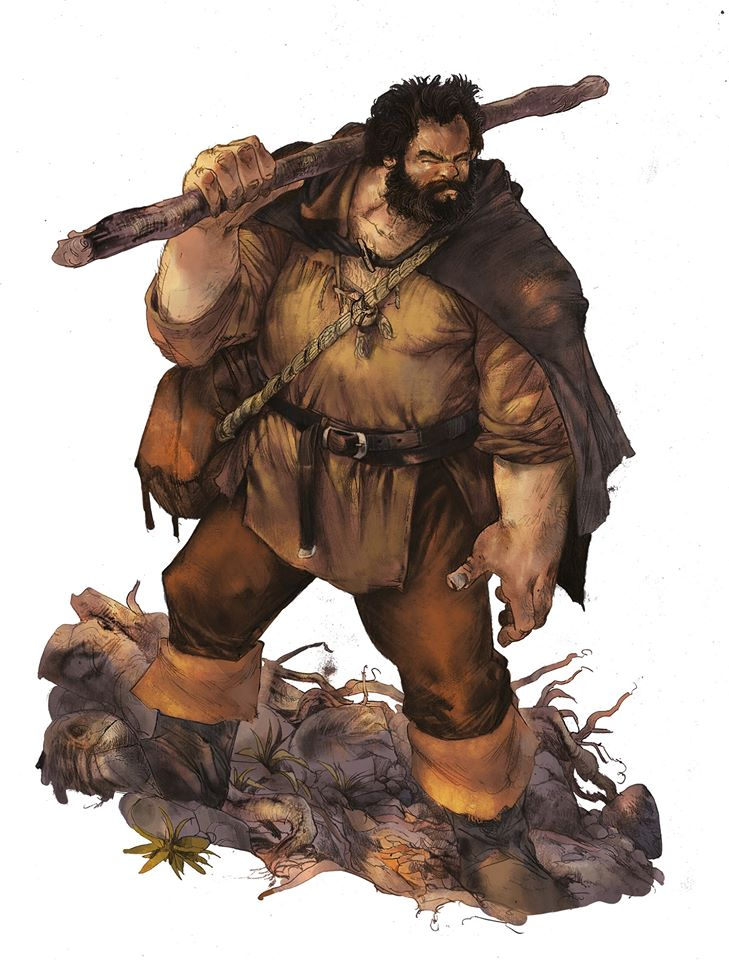
\includegraphics[width=0.48\textwidth]{02kins/img/19uman_monk.jpg}
\end{figure}

\subsection*{Traits}
The nomad kin is known for their survival and adaptability, and your uman character receives the following traits:

\subparagraph{Ability Score Increase} Two different ability scores of your choice are increased by 1.

\subparagraph{Age} Umans reach adulthood in their late teens and live less than a century, if they manage to survive that long.

\subparagraph{Alignment} Umans tend to no particular alignment, but they do have a penchant for community and justice, and tend to the indigo tide.

\subparagraph{Size} Umans vary widely in height and build, from barely 1.5 meters to well over 1.8 meters tall.
Regardless of your position in that range, your size is Medium.

\subparagraph{Speed} Your base walking speed is 9 meters.

\subparagraph{Languages} You can speak, read, and write the nomad tongue, and an additional language of your choice.
You can also read and write the traveller's cant, a set of writings and symbols created by your kin to help and communicate with each other.

\subparagraph{Learned Durability} You are competent in the Survival skill.

\subparagraph{Relentless Endurance} When you are reduced to 0 hit points but not killed outright, you can drop to 1 hit points instead.
You can't use this feature again until you finish a short rest.

\begin{figure}[!t]
    \centering
    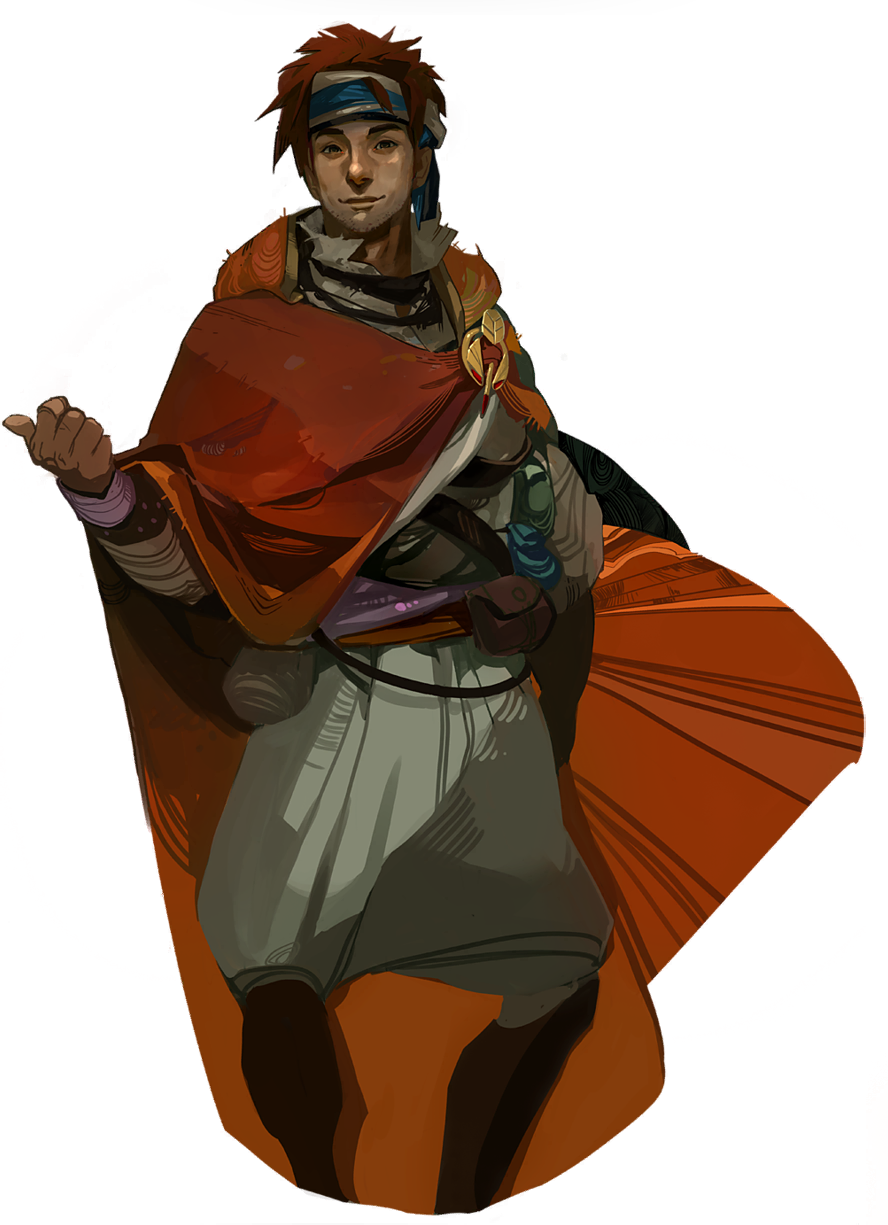
\includegraphics[width=0.48\textwidth]{02kins/img/19uman_nomad.png}
\end{figure}

\subsubsection{Common Nomad}
While umans are known to be extremely adaptable to extreme habitats, most don't stay at one place for enough time to acquire this specialty and remain, for lack of a better word, common.
In stark contrast with their name, each of these umans is unique and as such your features are specially dynamic.

\subparagraph{Languages} You can read, write and speak one additional language of your choice.

\subparagraph{Skills} You gain competence in one skill of your choice.

\subparagraph{Trained} You gain competence with one simple or martial weapon of your choice.

\subparagraph{Handy} You gain competence with a set of artisan's tools of your choice.

% \subparagraph{Feat} You gain one feat of your choice.

\subsubsection{Frostburn Nomad}
With skins ranging from pale blue to light purple, and hair shades from the lightest of white to deep brown colors, the Frostburn are a kin that comes from a troupe of umans that managed to survive in the lands beyond the wall of ice and stone, and beyond the reach of most coldblood beasts and nimrods.
%These umans tend to dress with the bones and furs of the creatures they hunt, using their inventiveness to craft clothing to intimidate and scare rather than protect against cold, since their thick skins already manage this task effortlessly.

\subparagraph{Ability Score Increase} Your Constitution score is increased by 1.

% \subparagraph{Menacing} You are competent in the Intimidation skill.

\subparagraph{Born Hunter} You are competent with clubs, daggers, spears, and barbed spears.

\subparagraph{Thick Skin} %You are naturally acclimated to cold environments and don't need sources of heat to survive in all but the most extreme cold.
You are resistant to cold damage.%, and remain unaffected by cold environments.

\subparagraph{Ice Shell} As two actions, you can grow a thick layer of ice around your body to protect you.
You gain resistance to piercing and slashing damage and vulnerability to bludgeoning damage for a number of turns equal to your Constitution modifier (Minimum of 1).
Additionally, any creature that attacks you with a melee attack during this time suffers 1d4 piercing damage.
You can use this trait once per short rest.

\subsubsection{Boggart}
Boggarts are umans that live in the swamps and marshes of Yuadrem.
Boggarts are generally tall, slim, and amber-skinned, with eyes of hazel or brown.
Their hair ranges from black to dark brown, but most shave off all their hair.
These umans are craftier than the average, and are known to prepare complex traps and mechanisms to protect their communities or alert them of imminent danger.

\subparagraph{Ability Score Increase} Your Wisdom score is increased by 1.

\subparagraph{Bog Swimmer} Boggart tactics usually include a good dose of swimming through less than cooperative waters.
You have a swimming speed of 9 meters.

\subparagraph{Swamp Life} You have advantage on saving throws against poison and diseases, and you have resistance against poison damage.

\subparagraph{Stealthy Hunter} You are competent with blowguns, nets, and bolas.
% You also are proficient with a Poisoner's kit.

\subsubsection{Cursed Kin}
It is said that the umans who remain in the place of their arrival start showing their true form.
While the accuracy of this statement remains untested, it is true that those who stay in the forbidden lands do show strange changes to their appearance.
Large, black horns grow on their heads, their skin and eyes turn into a very pale shade, and their bodies grow.
While most cursed kin do act more menacing and violent than the average uman, it is likely that this is a side effect of their harsh homeland more than a natural development in their minds.

\subparagraph{Size} Unlike most nomad kin, you stand between 2.1 and 2.4 meters tall and weight between 140 and 170 kg.
Your size is medium.

\subparagraph{Ability Score Increase} Your Strength score is increased by 1.

% \subparagraph{Natural Athlete} You have proficiency in the Athletics skill.

\subparagraph{Abyssal Resistance} You have resistance to fire damage.

\subparagraph{Unholy Fortitude} Your hit point maximum increases by an amount equal to your number of hit dice.

\subparagraph{Ram} Your horns are a natural weapon, which you may use use to make unarmed strikes.
If you hit with them, you deal bludgeoning damage equal to 1d4 + your Strength modifier, instead of the damage normal for an unarmed strike.

\subparagraph{Powerful Build} You count as one size larger when determining your carrying capacity and the weight you can push, drag or lift.

\begin{figure}[!b]
    \centering
    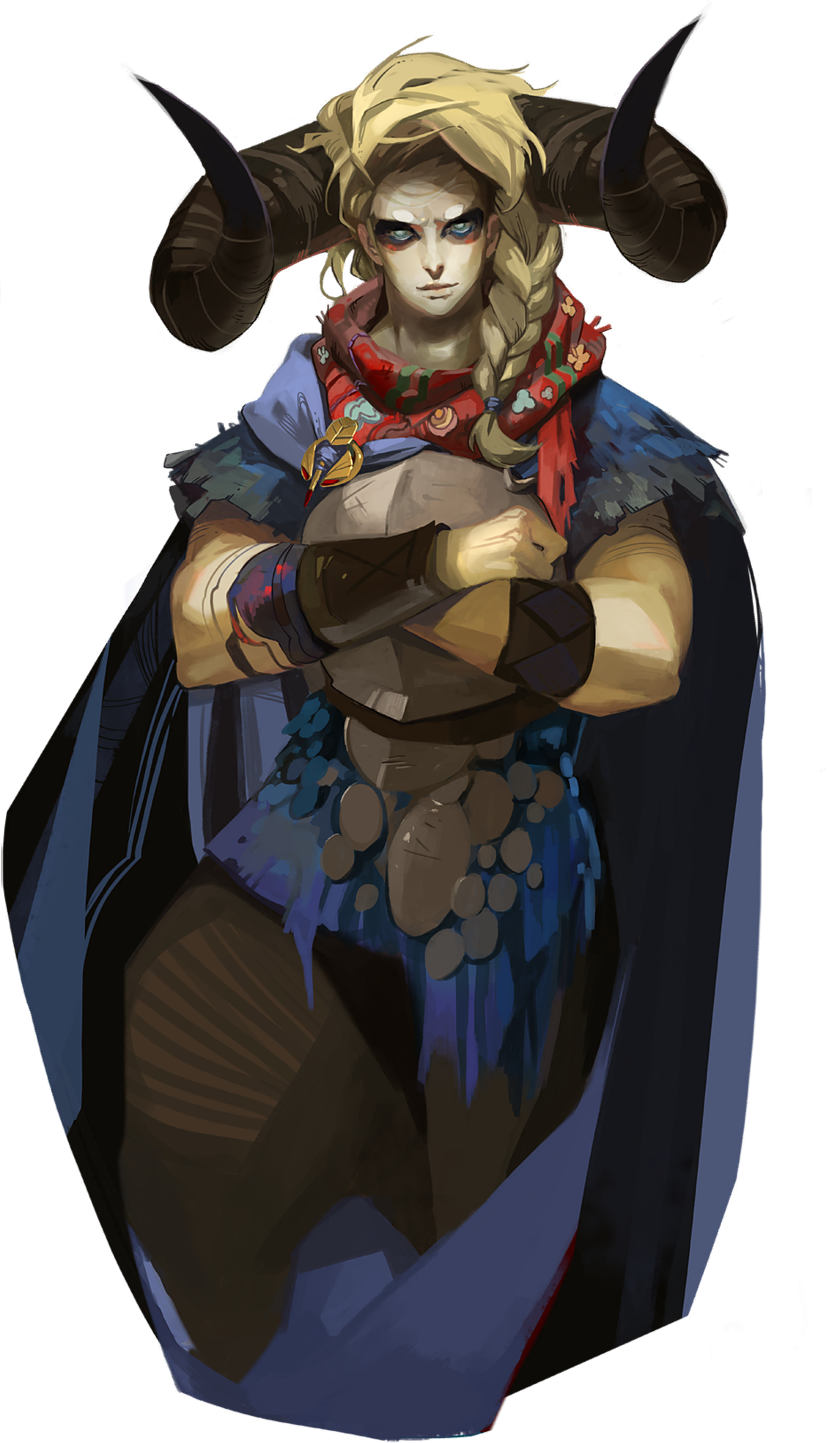
\includegraphics[width=0.48\textwidth]{02kins/img/19uman_cursed.png}
\end{figure}
\end{linenumbers}

% % !TEX root = ../main.tex
% TODO: GENERAL CHECKUP NEEDED

\section{Storm Kin}
\begin{linenumbers}
\DndDropCapLine{A}{sk anyone anywhere and they will give}
\textit{you a list of the things and people they lost to the ash storm.
That blasted cloud covered the entirety of the continent, leaving none unscarred.}

\hspace*{\fill} --- Iitus the scholar, "Of War and Thunder".

As the schism progressed, when the spire started spewing forth smoke and lava into the world, an immense ash storm gathered around the volcano, discharging lightning into anyone foolish enough to approach it.
As the years passed, the storm slowly subsided, leaving behind a strange race of being composed of ash, smoke, and lightning.
These being were named the zaloths, or storm kin, who adapted surprisingly well to the many kins of Yuadrem, and quickly found their new place in the world.

\subsection*{Ethereal Appearance}
The zaloths are tempests given physical shape, and their form reflects this.
They are composed of ash smoke, with strange forces shaping them into humanoid form.
Born from storm, they are in constant turmoil, and lightning sparks and cackles incessantly inside their bodies.

It is social norm for zaloths to clothe themselves in linen wrappings to cover their bodies, and it is not unusual for them to wear clothes or armor over these wrappings.
When they were formed, they also took the qualar of the unfortunate sentient creatures that were atop or near the spire, thus retaining their sentience.

Zaloths are not known to age or reproduce, and as such it's hard to tell if they'll be able to survive too long as a species.
They are thus extremely appreciative of their chance to experience life on Yuadrem, and are commonly known to be existentialists, looking to maximize their experiences in number and intensity.

When a zaloth suffers a mortal wound it does not die in a traditional sense, but the matter composing its body coalesces into a zaloth quintessent, a small cloud of ash.
This cloud does not retain its sentience, but it is somewhat able to keep its memories and experiences, and eventually merges into the atmosphere, becoming part of Yuadrem in a sense.

\subsection*{Distributed and Nomadic}
While a small group of zaloths established themselves in the city of Jan'krug at the top of the spire, the vast majority of the storm kin immediately started roaming the world alone or in small groups, looking for experiences.
Due to this, it is very rare to encounter an established zaloth community or zaloths living permanently in a city or town.
Nowadays, they are found wondering the land in caravans, circuses or as lone adventurers, eternally seeking new experiences.

When a wandering zaloth group meets another, it is common for them to celebrate this encounter by throwing a party in commemoration of their common heritage.
During this event, the members of the different groups conduct a ritual known to them as the mingling, where they allow their bodies to fuse, and thus share with each other their memories and experiences.

\subsection*{Presence in the World}
Due to their rarity, the other kins generally treat them with wonder and even admiration.
Many schools of thought regard the zaloths as sages due to the wisdom obtained in their nomadic ways, and their unique viewpoint on life and the world is appreciated by any who seek knowledge.

This however does not mean that all zaloths describe themselves as savant.
On the contrary, some of them give in to their inherent chaotic nature and become agents of turmoil, seeking paramount experiences via extreme means.
While their methods are frowned upon by more orthodox zaloths, they are far from being a pariah; they engage in mingling as commonly as any other zaloth.

\subsection*{Life of Adventure}
Due to the existentialist nature of the zaloths, a life of adventure is the most natural lifestyle that comes to them.
However, most zaloths are far from reckless, and while they can find dangers in their travels, they are careful to avoid mortal danger.
To the storm kin, any zaloth's death is a tragedy, and they prioritize the life of any of their kin over that of all other creatures.

A traveling zaloth will try all sorts of activities, independent of their nature and intensity.
Ever seeking new experiences, it is equally likely to encounter a zaloth engaging in quiet appreciation of nature, martial combat against formidable enemies, or joining in on other species' religious rituals.
Or even all of these activities on the same day.

\subsection*{Zaloth Names}
Due to the special conditions to their coming into the world, zaloths are born without names.
A zaloth usually chooses a name for itself after years, decades or even centuries of travel, and while it is nameless it is referred to using a feat or special characteristic that defines it.
The names that a zaloth chooses are commonly taken from other cultures or carefully designed by it.

\paragraph{Names} Basks-in-the-Sun, City-Swimmer, Dreams-of-Sleep, Dusk-Skin, Far-From-Water, Forest-Child, Has-no-Regrets, Head-in-Clouds, Iron-Fists, Mumbles-when-Speaks, Sees-All-Colors, Six-Coins, Somber-Mind, Sleeps-with-Open-eyes, Stands-in-Shallows, Swift-Legs, Takes-in-Light.

\begin{figure}[!t]
    \centering
    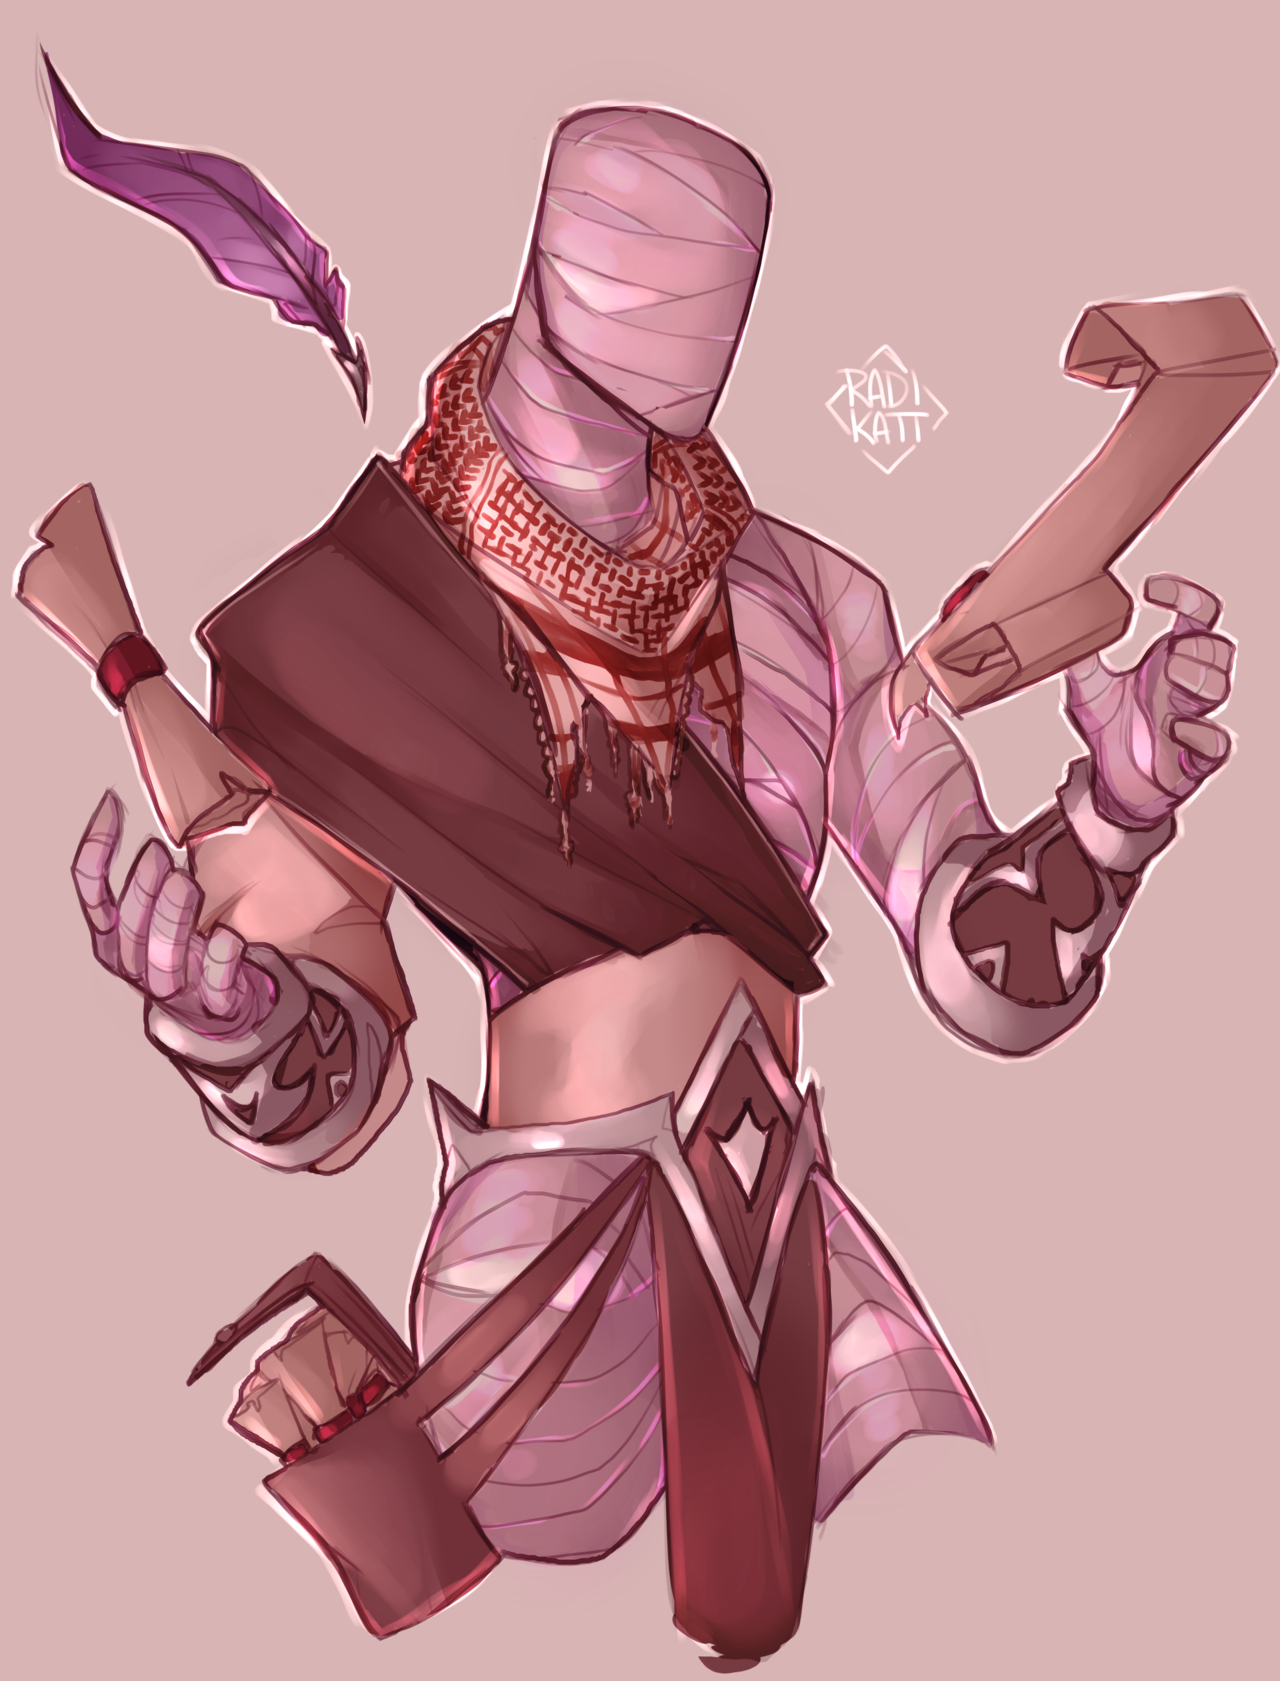
\includegraphics[width=0.48\textwidth]{02kins/img/20zaloth_scholar.png}
\end{figure}

\subsection*{Traits}
Your zaloth character has an assortment of traits related to its unique nature and nomadic lifestyle.
\subparagraph{Ability Score Increase} Your Charisma score increases by 1, and your Intelligence score increases by 1.
\subparagraph{Age} Born from an ash storm, a zaloth is thrust into adulthood, retaining some of the memories of the tall one from which it acquired its qualar as a blurry image.
Zaloths are not known to die from natural causes, and all of them are about 673 years old.
\subparagraph{Alignment} Most zaloth tend toward chaos, with little regard for the affairs of civilizations.
Due to their curious nature and lifestyle, zaloths move with the red tide.
\subparagraph{Size} Zaloths stand between 1.5 and 1.8 meters, and are practically weightless due to their unique composition.
\subparagraph{Speed} Your base walking speed is 9 meters.
\subparagraph{Dual Nature} You are both humanoid and elemental.
You can be affected by an effect if it works on either of these two creature types.
\subparagraph{Incorporeal} You are immune to poison damage, and cannot be affected by poison or disease.
You also don't need to eat or drink.
% \subparagraph{Hover} Instead of walking, your can choose to hover up to 1 feet over the ground.
% You can still be thrown into the ground if you are knocked prone, but you only need 5 feet of movement to stand up and don't provoke attacks of opportunity when you do so.
\subparagraph{Radiant} You give off dim light in a 3-meter radius and have disadvantage on Dexterity (Stealth) checks.
You cannot block this light with any clothing or armor.
\subparagraph{Telepathic} You can speak telepathically to any creature you can see within 9 meters of you.
Your telepathic utterances are in a language you know, and the creature understands you only if it knows that language.
Your communication doesn't give the creature the ability to respond to you telepathically.
\subparagraph{Silent Speaker} You can ignore the verbal components of spells.
\subparagraph{Languages} You can understand, read and write two languages of your choice, but you are unable to speak any language.
You can understand a very limited vocabulary of the old tongue, usually limited to individual words without context.

\subsubsection{Gale Zaloth}
Different zaloths have a stronger tendency towards different elements of the ash storm from which they were born.
Gale zaloths are attuned to the shifting, violent winds of the storm, and they reflect this with their erratic movements and shifting conversation subjects.
% A constant breeze can be felt around them, a grim reminder from the ash clouds.
\subparagraph{Ability Score Improvement} Your Dexterity score increases by 1.
\subparagraph{Stormbound} Wherever you go, you carry some of the storm with you.
A light breeze can be permanently felt in a 3-meter radius around you, moving in a random direction every turn.
The wind of this breeze displaces all smokes, gases, and very light objects inside its radius.
You can choose to end or restart this effect as a free action.
\subparagraph{Potent Quintessent} When you drop to 0 hit points, your desire to live manifests as a strong shockwave, sending any creature standing near you flying.
All creatures that stands in a 3-meter radius around you must succeed on a DC 16 Strength saving throw.
On a fail, a creature takes 1d6 force damage, is pushed 12 meters, and is knocked prone.
On success, a creature only takes half the damage, and isn't pushed or knocked prone.
You can use this ability once per long rest.
\subparagraph{Wind Given Form} You know the gust cantrip.
Once you reach 3rd level, you can cast the feather fall spell; you must finish a long rest in order to cast the spell again using this trait.
Once you reach 5th level, you can cast the dust devil spell as a 2nd level spell, requiring no material components; you must finish a long rest in order to cast the spell again using this trait.
Charisma is your spellcasting ability for these spells.

\subsubsection{Thunder Zaloth}
Thunder zaloths are attuned to the fleeting, fierce lightning.
They reflect this relation with their quick movements and sparking personalities.
\subparagraph{Ability Score Improvement} Your Charisma score increases by 1.
\subparagraph{Instant Step} You can expend your movement and a bonus action to transport instantly to a location up to your movement speed away that you can see.
Any creature standing in the straight line between the two positions must succeed on a DC 12 Constitution saving throw, taking 1d8 lightning damage on a failure.
You can do this a number of times equal to your Charisma modifier (Minimum of 1), and you regain all expended uses when you complete a short or long rest.
\subparagraph{Elemental Resistance} You have resistance to lightning damage.
\subparagraph{Electricity Given Form} You know the shocking grasp cantrip.
Once you reach 3rd level, you can cast the thunderwave spell as a 2nd level spell; you must finish a long rest in order to cast the spell again using this trait.
Once you reach 5th level, you can cast the shatter spell as a 2nd level spell; you must finish a long rest in order to cast the spell again using this trait.
Charisma is your spellcasting ability for these spells.

\subsubsection{Ash Zaloth}
Ash zaloths are attuned to the destructive force of the spire, given form in the ash storm.
They embody the violence of the storm, and have affinity towards inflicting and receiving pain.
\subparagraph{Ability Score Improvement} Your Strength score increases by 1.
\subparagraph{Storm Conduit} The chaos of combat stirs your inner storm.
Once per round, you can deal an extra 1d4 fire damage to one creature you hit with an unarmed strike or an attack made with a metal weapon.
At 11th level, this damage increases to 2d4.
You can do this a number of times equal to your Charisma modifier (Minimum of 1), and you regain all expended uses when you complete a short or long rest.
\subparagraph{Elemental Resistance} You have resistance to fire damage.
\subparagraph{Flame Given Form} You know the produce flame cantrip.
Once you reach 3rd level, you can cast the burning hands spell as a 2nd level spell; you must finish a long rest in order to cast the spell again using this trait.
Once you reach 5th level, you can cast the Aganazzar's scorcher spell as a 2nd level spell; you must finish a long rest in order to cast the spell again using this trait.
Charisma is your spellcasting ability for these spells.

\subsubsection{Hail Zaloth}
Rarest of their species, the hail zaloths are the youngest of the zaloth, embodying the freezing hail into which the ash storm eventually decanted.
While still existentialist, they approach their curiosity in a calmer fashion, preferring the stillness of nature to the rowdiness of civilized society.
\subparagraph{Ability Score Improvement} You Wisdom score increases by 1.
\subparagraph{Cryogenic Stillness} You can choose to temporarily freeze your entire body, granting you extreme resilience.
As a free action or reaction, you can instantly freeze, granting you immunity to slashing, piercing, and bludgeoning damage, apart from resistance to acid, force, lightning, necrotic, and thunder damage.
You also gain vulnerability to fire damage.
You are also affected by the slow spell for the duration of this trait without the possibility to roll saving throws.
You can maintain this effect for a number of turns equal to your Charisma modifier (minimum of 1), and must finish a long rest in order to use this trait again.
\subparagraph{Elemental Resistance} You have resistance to cold damage.
\subparagraph{Ice Given Form} You know the frostbite cantrip.
Once you reach 3rd level, you can cast the ice knife spell as a 2nd level spell; you must finish a long rest in order to cast the spell again using this trait.
Once you reach 5th level, you can cast the icy surface spell as a 2nd level spell; you must finish a long rest in order to cast the spell again using this trait.
Charisma is your spellcasting ability for these spells.

\begin{figure}[!b]
    \centering
    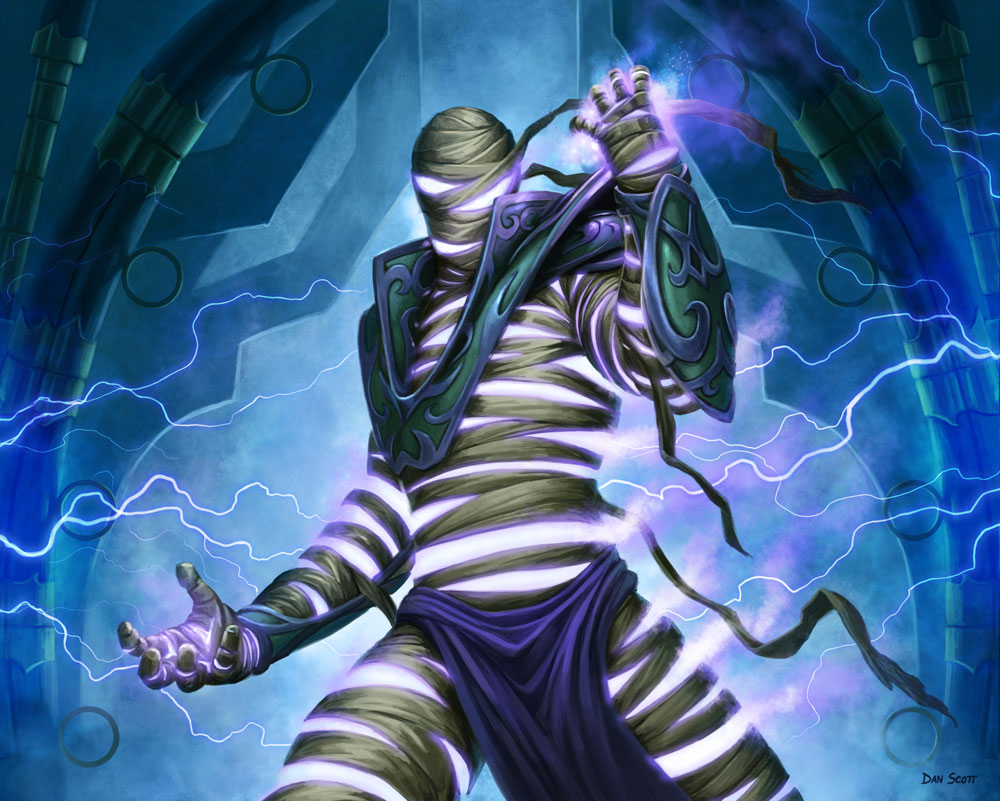
\includegraphics[width=0.48\textwidth]{02kins/img/20zaloth_thunder.jpg}
\end{figure}

\end{linenumbers}

% % TODO: GENERAL CHECKUP NEEDED

\section{Retainer Kin}
\begin{linenumbers}
\DndDropCapLine{T}{hey are the last kin created by our}
\textit{creators, and as such are related to us gats, irds, and oths.
It is our duty to provide them the nourishing that our shared parents denied them.
They are, after all, our younger siblings.}

\hspace*{\fill} --- Kosmael, founder of the church of Jismuah.

After the schism, as the storm that covered the tall kin's tiding dispersed, many dark secrets were revealed.
Among these sins, the existence of the quies, or retainer kin, was of special note.
The retainer kin is a fully sentient species which, unlike the other created by the tall kin, was forced into servitude, unable to comprehend what it is to roam free or even the existence of a world outside of Jan'krug.

At some point after the tall kin secluded themselves in their mountaintop city, they decided to create this slave race to focus solely on their studies and rituals.
The quies, not understanding what freedom is, remained immersed in their tasks for centuries, continuing even after the tall ones vanished.
They continued in this meaningless loop until gat expeditioners found them, still locked into servitude to their dead masters, and showed them a life unbound by chains.

\subsection*{Designed with a Purpose}
Such as gats, irds, oths, and marsets, the quies were created by the tall kin.
Unlike them, the quies were formed from a blend of organic and inorganic materials.
Their bodies are made from a blend of flesh and wood, with root-like cords infused with strange fluids serving as muscles, wrapped around a framework of bone and flesh.

Armored plates form a protective outer shell and reinforce joints.
Quies' faces are simply a collection of holes located where sensory organs would normally be, but each has a custom made qualar mask integrated into this outer shell.
These masks usually contain very intricate detail, and seem to be made with an almost ardent passion.

\subsection*{Functionalist at Heart}
The quies were built to serve.
For the first centuries of their existence, the retainer kin had a clearly defined function and were encouraged to focus purely on that role.
While they now might have freedom, many still struggle both to find a place in the world and to relate to the creatures of it.

The typical quies show little emotion.
Many of them embrace a concrete purpose-such as protecting allies, completing a contract, or exploring a land-and embrace this task as they once did.
However, there are quies who delight in exploring their feelings, their freedom, and their relationships with others.
The race was first welcome to Yuadrem by the church of Jismuah, and many embraced faith and mysticism, seeking higher purpose and deeper meaning.

\subsection*{Life of Subservience}
The quies are the sentient beings that spent the most time living alongside the tall kin, and as such they are highly sought after by scholars studying them.
While a quies can describe in great detail the daily life of a tall one, their subservient nature inhibited their curiosity.
Not one quies is known that can recall the rituals performed by the tall kin, and most can't even tell anything about their masters other done the tasks they performed for them.

Like the zaloths, the quies are unable to reproduce by any mean, which is probably by design.
This, combined with the fact that their creators have almost completely disappeared from Yuadrem, makes their chances of survival as a species look very grim.
This is countered however by the fact that, as their creators, quies don't seem to age at all.

\subsection*{New Beginnings}
After leaving Jan'krug, the retainer kin had a very hard time adapting to the world.
Some dedicate themselves to continuing their skill under a new patron, failing to leave behind their lives as servants.
Others managed to learn independence, but could not abandon their craft, and became renowned artisans or merchants, being compared by many even to gat artisans.

The quies that managed to completely break free from their bindings are regarded as special by the other members of their species, and they are met with both reverence and jealousy.
These quies usually become adventurers, where they can blend their newfound curiosity with their armored bodies.
Some take the plight of their kin into their hearts, and spend their lives trying to find the last remaining tall ones, aiming to learn how to create more of their own.

\subsection*{Quies Names}
As far as is known, no tall one ever gave a name to a quies.
Most of the retainer kin simply refer to themselves by their job, or by a name given to them by others.
However, the quies that manage to escape their shackles and take a life of wandering are very appreciative of being given the freedom to pick their own names.
Once chosen, a quies will guard their name with great jealousy, only sharing it with whom they trust the most.

\paragraph{Names} Ba, Bal, Dreth, Eth, Feather, Fish, Gakn, Green, I, Jan, Jatherlin, Loth, Risz, Seed, Sekru, Stand, Swim, Tis, Tlekeloo, Tlos, When, Yu, Zash.

\begin{figure}[!t]
    \centering
    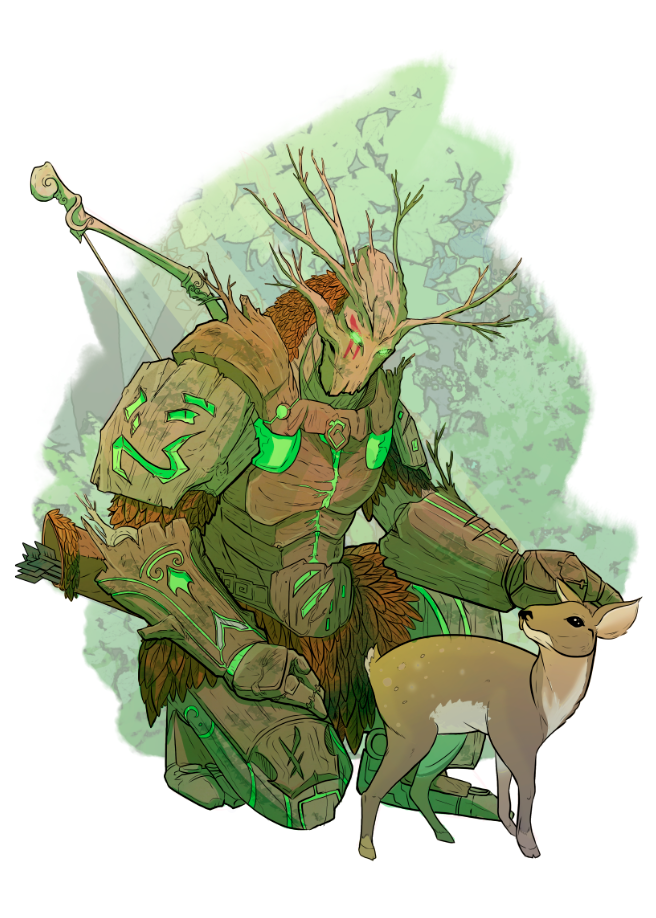
\includegraphics[width=0.48\textwidth]{03kins/img/quies_druid.png}
\end{figure}

\subsection*{Traits}
Designed for efficiency, your quies character has the following traits:
\subparagraph{Ability Score Increase} Your Constitution score increases by 1.
\subparagraph{Age} Every quies is somewhere between 673 and 890 years old, but their memories before the schism are vague and unreliable.
Since they've shown no sign of deterioration due to age, quies are assumed to be immortal.
\subparagraph{Alignment} Most quies take comfort in order and discipline, tending toward law and neutrality, but some have chosen a new morality based on the experiences of their independent life.
They are a blank slate, and do not tend to any particular tide as a species.
\subparagraph{Size} Quies are of formidable size, standing between 1.8 and 2.25 meters tall.
Your build is determined by your subrace.
Your size is medium.
\subparagraph{Speed} Your base walking speed is 9 meters.
\subparagraph{Dual Nature} Due to your manufactured nature, you are both humanoid and construct.
You can be affected by an effect if it works on either of these two creature types.
\subparagraph{Quies Resilience} You were created with fortitude in mind.
You have advantage on saving throws against being poisoned, and you have resistance to poison damage.
\subparagraph{Immutable Form} Protected by the strange designs of the tall kin, you have advantage on saving throws against effects that would alter your form.
\subparagraph{Integrated Protection} Your body has built-in defensive layers, which can be enhanced with armor:
\end{linenumbers}
\begin{itemize}
    \item You gain a passive +1 to Armor Class.
    \item You can only don armor with which you have proficiency.
    To don armor, you must incorporate it into your body over the course of 4 hours, during which you remain in contact with the armor.
    To doff armor, you must spend 1 hour removing it.
    \item While you live, your armor can't be removed from your body against your will.
\end{itemize}
\begin{linenumbers}
\subparagraph{Mountain Built} You are impervious to most effects of altitude, except for those related to cold.

\subsubsection{Quies Operative}
You were designed with a certain specialized function in mind.
You might be a carpenter, a cartographer, or an entertainer, to name a few possibilities.

Operatives are the most common of the quies, yet each is of unique design.
Your build is dependent on the task you were designed for, and you can be as light as 70 kg to as heavy as 150 kg.
\subparagraph{Ability Score Increase} Any two ability scores between Strength, Dexterity, Intelligence, Wisdom, or Charisma of your choice increase by 1.
\subparagraph{Integrated Tool} You have expertise with one set of artisan's tools or one instrument of your choice, apart from smith's tools.
This tool or instrument is integrated into your body, and is related to what was your purpose when you lived in Jan'krug.
You must have your hands free to use this integrated tool.
\subparagraph{Specialized Design} You have expertise with one skill of your choice.

\subsubsection{Juggernaut}
While many tall ones were more than capable of dealing with heavy lifting, they designed this branch of quies for fulfilling these kinds of tasks in conditions less ideal for a tall one, or simply to work in cooperation with them.
Juggernauts have a large frame and powerful build, and can weigh up to 230 kg.
% While these quies were not specifically designed to fight, they usually prove more than capable of melee combat.
\subparagraph{Ability Score Increase} Your Strength score increases by 2.
\subparagraph{Hard Fists} Your arms and fists are lined with obsidian, a specially hard stone from the higher parts of the spire.
When you hit with an unarmed strike, you can deal 1d4 + your Strength modifier bludgeoning damage, instead of the normal damage for an unarmed strike.
% Feat: Replace obsidian with quartz for even stronger fists.
\subparagraph{Long-Limbed} When you make a melee attack on your turn, your reach for it is 1.5 meters greater than normal.
\subparagraph{Powerful Build} You count as one size larger when determining your carrying capacity and the weight you can push, drag, or lift.

\begin{table*}[b]%
    \begin{DndTable}[width=\linewidth]{X}
        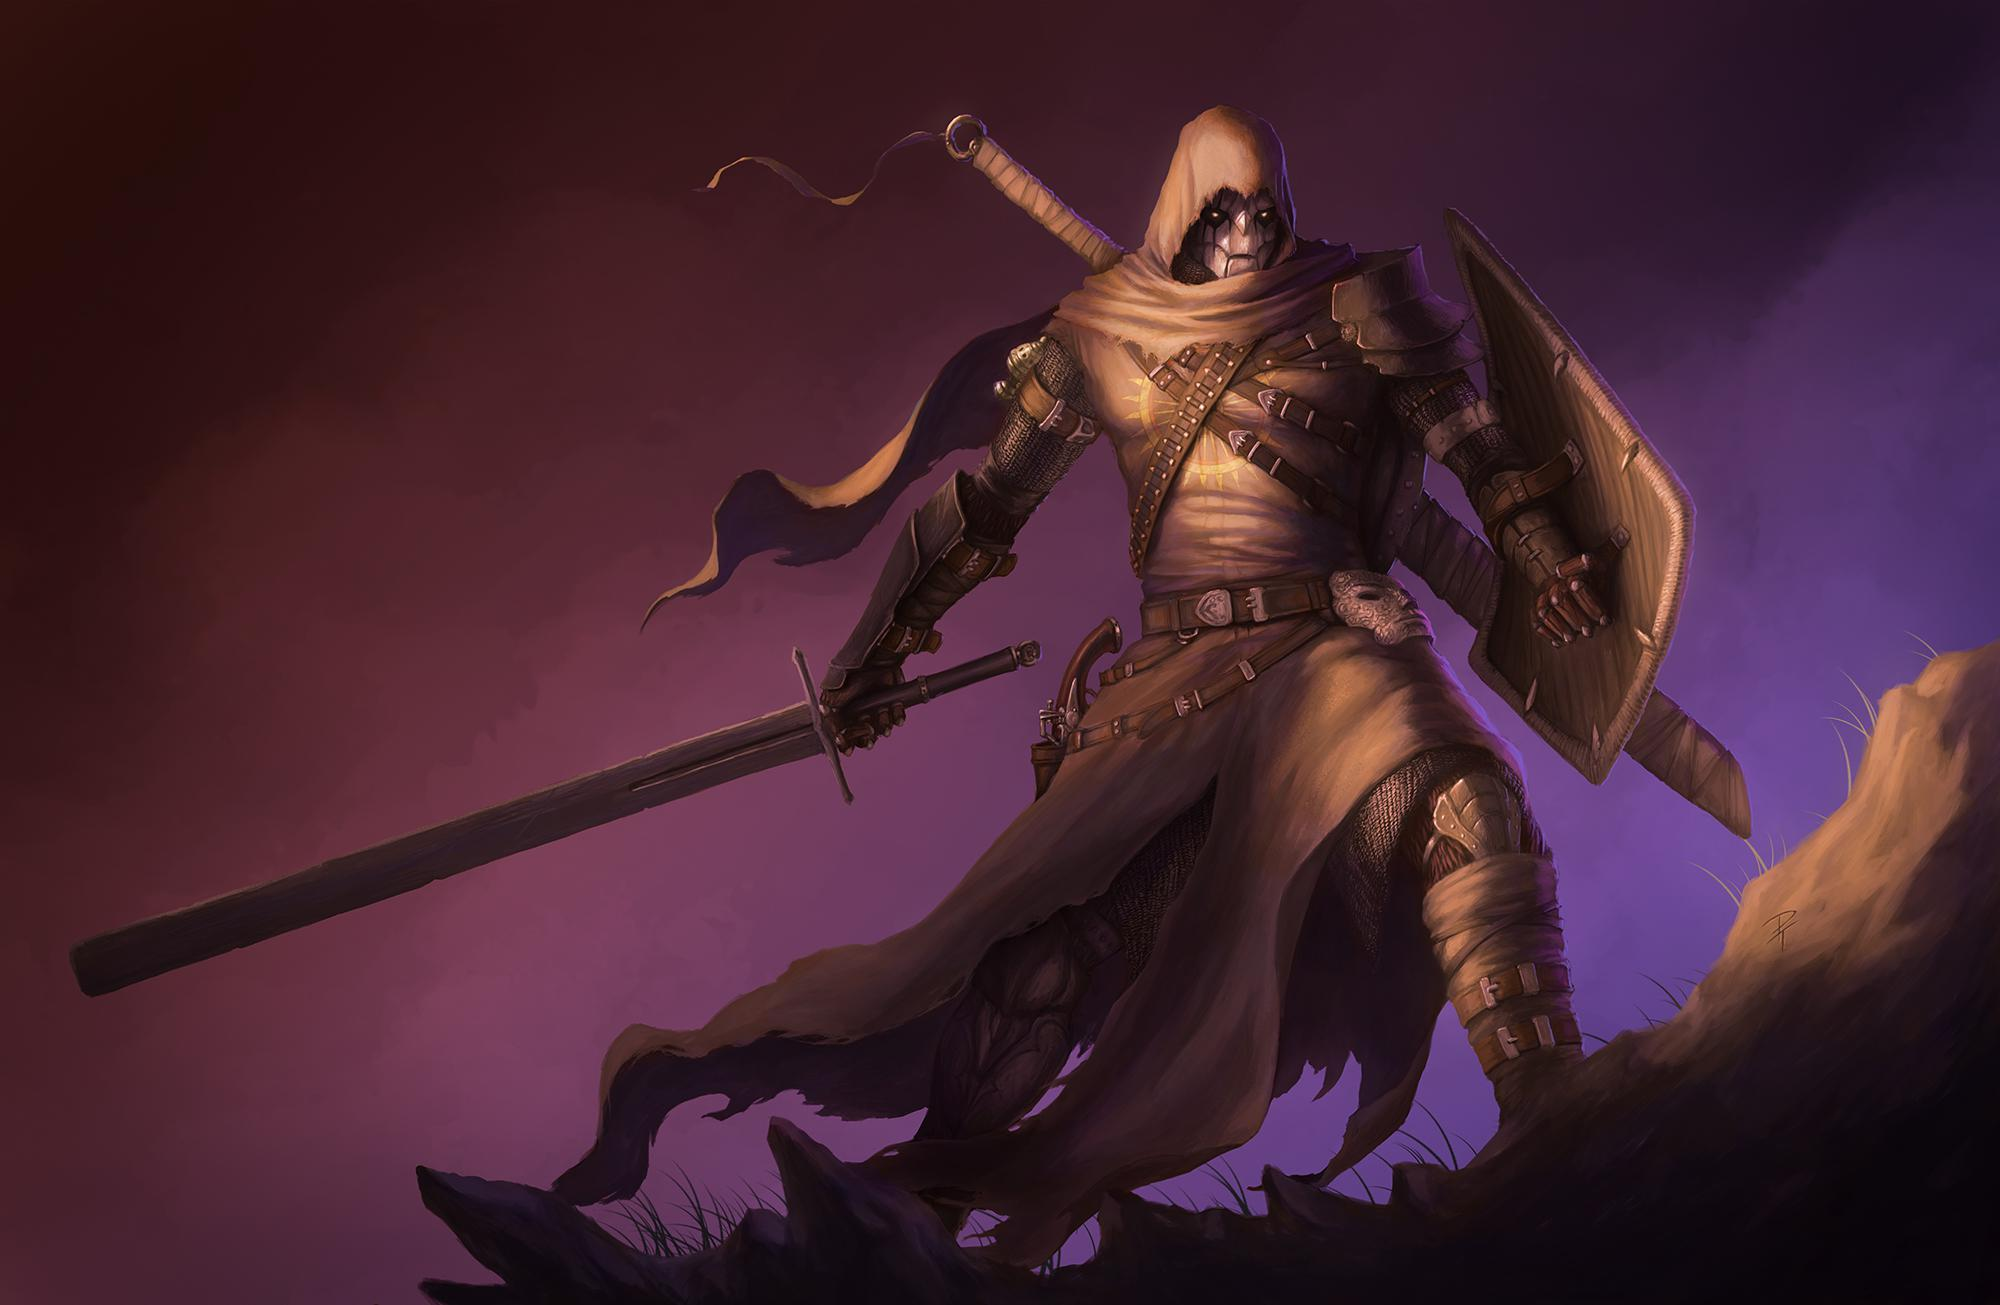
\includegraphics[width=0.98\textwidth]{03kins/img/quies_executioner.jpg}
    \end{DndTable}
\end{table*}

\subsubsection{Slag Worker}
Even with the adaptable form of the tall kin, not even them can survive being drenched in lava.
Consequently, when their rituals required them to work inside the volcano, they created the slag workers, quies designed specifically for this purpose.
Built to work under extreme pressure, the carapace of the slag workers is a thick layer made from rhyolite.
While the rock deforms and contorts under lava, it completely blocks the quies from the liquid and its heat.
Even the qualar of these quies is infused with the rock, to completely isolate them from their environment.
\subparagraph{Ability Score Increase} Your Strength score increases by 1, and Constitution score increases by 1.
\subparagraph{Heavy Plating} This trait replaces integrated protection.
Your Armor Class is 16 + your proficiency bonus, and you have disadvantage of Dexterity (Stealth) checks.
For all intends and purposes your armor is considered Heavy Armor, and it cannot be removed from your body in any way while you are alive.
This armor is of a light pink or gray color, and is some cases contains vugs filled with obsidian or quartz.
\subparagraph{Specialized Worker} You are resistant to fire damage.
You are also able to enter bodies of lava or magma, sinking at a speed of 5 feet per turn and not suffering any damage while inside.
For the purposes of moving, lava and magma counts as difficult terrain for you.
You still need to breathe, and you must follow the normal rules for holding your breath while submerged in the sizzling hot liquid.
\subparagraph{Defensive Stance} As a bonus action, while you have one hand free, you can choose to enter a defensive stance.
You add your proficiency bonus to your armor class until the start of your next turn.
this trait a number of times equal to your Constitution modifier (minimum of 1), and must take a short or long rest before doing so again.
\end{linenumbers}

